%!TEX encoding = UTF-8

\chapter{Tool Use Affordances}
\label{chap:tool}

In this chapter, we present a computational model of affordances capable of dealing with multiple objects (see Fig.~\ref{fig:tool:tools_computational_model}), giving rise to a \emph{tool use} behavior.
This skill is useful to operate in complex manipulation tasks typical of human-like environments.

\begin{figure}[h]
\newcommand{\myscaleaffmodels}{0.6}
\centering
\begin{tikzpicture}[scale=\myscaleaffmodels, every node/.style={transform shape}]
\montesanoAE
\saponaroManipulatorUseBox
\end{tikzpicture}
\caption{Computational model of affordances for dealing with multiple objects and tool use.
In this chapter, the manipulator corresponds to the held object (i.e., tool) or to the robot hand.}
\label{fig:tool:tools_computational_model}
\end{figure}

The concept of tool use has been studied extensively in cognition research of humans and other animals~\cite{beck:1980,st_amant:2008:animal}.
Beck defines it as
``[\dots] the external employment of an unattached environmental object to alter more efficiently the form, position, or condition of another object, another organism, or the user itself when the user holds or carries the tool during or just prior to use and is responsible for the proper and effective orientation of the tool'' \cite[p.~10]{beck:1980}.

We accomplish a tool use behavior with our computational model through reasoning, learning and a developmental approach.

In terms of reasoning, we have the robot interpret the possibilities offered by \emph{multiple entities} in a joint way.
In particular, the robot interprets the possibilities permitted by a \emph{manipulator} onto an \emph{acted object}.
By manipulator, we refer to a first, grasped object which acts as a tool (also known as held or intermediate object), being located in the agent's hand; we also use the term manipulator to indicate the bare hands of the robot with a particular aperture of the fingers, when we study the transition from hand to tool affordances.
By acted (or primary) object, we refer to the target object in the scene over which the action is exerted.
A key aspect of our system is that it analyzes the relationship between \emph{sub-parts} of objects: not only looking at the level of their entirety, but also at their constituent sub-parts, such as the handle part or the effector/tip part of objects.

For \emph{learning} tool affordances, we evaluate different computational models, in particular different \ac{BN} structures and parameters, for evaluating
the capability of predicting effects from previously unseen data (generalization), and the possibility of transfering predictions from robot simulation to the real world.

Finally, we propose a method for learning the affordances of different robotic hand postures, investigating the \emph{developmental link} from hand affordances~(i.e., action possibilities by using the hands) to tool affordances~(action possibilities by using tools).

This chapter is the subject of the following publications:
\listPublicationsTools

The outline of this chapter is as follows.
Sec.~\ref{sec:tool:motivation} gives motivations for developing a tool use behavior in robots;
Sec.~\ref{sec:tool:related_work} lists related work from the literature;
Sec.~\ref{sec:tool:approach} presents our proposed approach.
In Sec.~\ref{sec:tool:results} we report the experimental results,
and finally in Sec.~\ref{sec:tool:conclusions} we draw our conclusions and possible future extensions.

%%%%%%%%%%%%%%%%%%%%%%%%%%%%%%%%%%%%%%%%%%%%%%%%%%%%%%%%%%%%%%%%%%%%%%%%%%%%%%%%
\section{Motivation}
\label{sec:tool:motivation}

Many important human behaviors require putting (multiple)~objects in such a way that they are in physical contact with each other.
A fundamental cognitive ability to master such skill is to understand the relationships between the physical properties of the objects' surfaces that enter into contact, i.e., \emph{\intobj} affordances or mutual affordances among objects.
For instance, to pile objects we must put into contact their flat surfaces to assure stability~(see Fig.~\ref{fig:tool:behaviors_intobj:pile});
to bring objects that are out of reach from our arms closer to us, we pull them with elongated objects~(see Fig.~\ref{fig:tool:behaviors_intobj:faraway});
to fit objects together we match concave parts on one object to corresponding convex parts on the other~(see Fig.~\ref{fig:tool:behaviors_intobj:fit}).

\begin{figure}
\centering
\subfloat[][Making a pile.]
{ 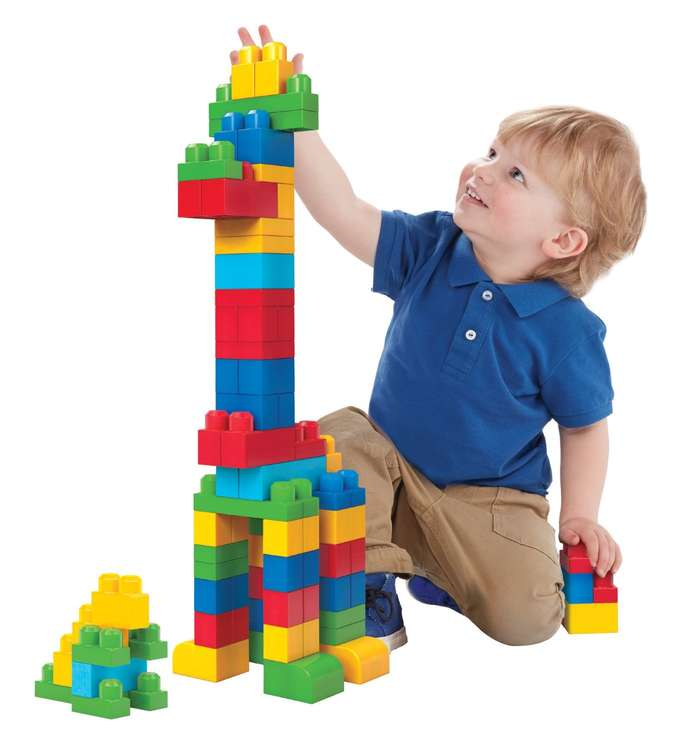
\includegraphics[width=0.27\textwidth]{building-blocks-for-kids-resized} \label{fig:tool:behaviors_intobj:pile} } \quad
%
\subfloat[][Reaching for faraway objects.]
{ 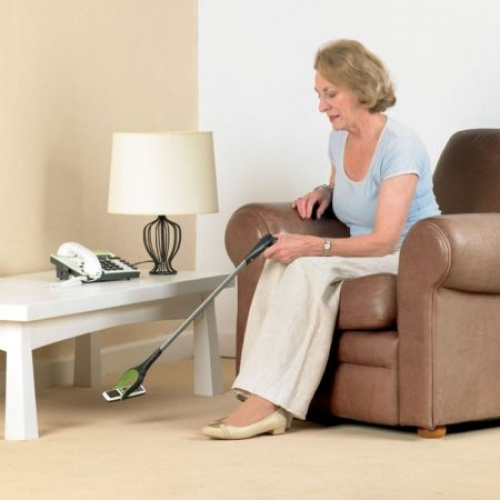
\includegraphics[width=0.27\textwidth]{revoreach_grip_lock_reacher} \label{fig:tool:behaviors_intobj:faraway} } \quad
%
\subfloat[][Fitting.]
{ 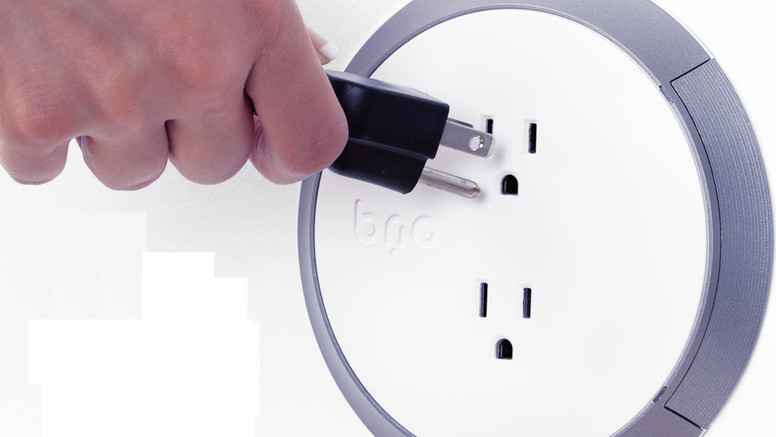
\includegraphics[width=0.27\textwidth]{placing_electrical_plug} \label{fig:tool:behaviors_intobj:fit} }
\caption{Examples of human behaviors that involve multiple objects in relationship with each other.}
\label{fig:tool:behaviors_intobj}
\end{figure}

In humans, the first tools are one's own hands.
Learning the affordances of the hands~(i.e., what actions one can do with them, what effects one can obtain) is a long developmental process that begins in infancy~\cite{egibson:1994,james:2010:icd}.
At~6 months of age, infants already manipulate objects in a differentiated manner depending on the object's properties~\cite{bushnell:1993:child}.
The process continues during childhood through exploration of different actions and different objects~\cite{rosenblatt:1977:bioplay,rosenbaum:2009}.
In essence, children achieve \intobj{} and functional tool use reasoning abilities over several stages~\cite{lockman:2000:childdev,szokolszky:2010,lobo:2013:ibd,fagard:2014:emergence}.
The knowledge previously acquired by babies during manual exploration of objects is likely to play a role in tool use.
Definitely, one of these roles is that the increased hand dexterity acquired during development allows the child to correctly grasp, manipulate and orient a tool; however, another role may be that the child ``sees'' in the shapes of some tools relevant characteristics that remind the child of previously used shapes of the own hands~(although no experimental evidence of this perceptual skill has been provided in the developmental psychology literature, as far as we know).

Typically, a manipulative robot operates on external objects by using its own hands~(or similar end-effectors), but in some cases the use of tools may be desirable.
For instance, if the robot has to use certain objects which are not reachable (due to geometric workspace constraints), tools may be a convenient way to extend the length of robot limbs, thus permitting the robot to reach for far objects.
The advantage of modeling \intobj{} affordances (i.e., affordances among multiple objects) is that this permits to infer
(i)~affordances of acted objects,
(ii)~affordances of manipulator (held) objects, and
(iii)~affordances of the interaction between held and acted objects.
Our model can be used
to predict effects given both objects and the performed action (i.e., effect prediction), or choose the best manipulator object or tool to achieve a goal (i.e., tool selection), or choose the best action given the available objects and a desired effect (i.e., action selection, which is particularly useful for planning complex actions made up of many simple steps, as we will see in Ch.~\ref{chap:poeticon++_case_study}).
In general, the evaluation tasks that we devise aim to test
the capability of predicting effects from previously unseen data (generalization), and the possibility of transfering predictions from robot simulation to the real world.

Inspired by the above observations in developmental psychology, and motivated by a need of autonomous robotic systems, we investigate the following aspects related to tool use on robots:
\begin{itemize}
\item we design a \emph{reasoning model} of visual \intobj{} affordances, namely a model that deals with the relationships between (i)~pairs of objects, (ii)~sub-parts of said objects;

\item we devise a method to \emph{learn} \intobj{} affordances, by designing and evaluating variations of the above model, both specified \apriori{} or automatically obtained from experimental data via \StructureLearning{} (see Sec.~\ref{sec:background:theory:structure_learning});

\item we make a robot learn the affordances of different hand postures and, having done that, we investigate the \emph{developmental link} from hand affordances (i.e., action possibilities by using the hands) to tool affordances (action possibilities by using tools).
\end{itemize}

About the model, we specialize our system for visual robot affordances (introduced in Sec.~\ref{sec:platform:software_architecture}) so that it is able to process multiple simultaneous objects, their mutual relationships, and the relationships between object sub-parts (e.g., handle part and effector part).

In terms of learning, we compare different \ac{BN} structures and parameters, and we evaluate them for the tasks of
(i)~predicting effects from previously unseen data (generalization), and
(ii)~the possibility of transfering predictions from robot simulation to the real world.

About the link from hands to tools, we explore how a learned representation of hand affordances can be generalized to estimate the affordances of tools
which were never seen before by the robot.

%%%%%%%%%%%%%%%%%%%%%%%%%%%%%%%%%%%%%%%%%%%%%%%%%%%%%%%%%%%%%%%%%%%%%%%%%%%%%%%%
\section{Related Work}
\label{sec:tool:related_work}

This section overviews related work about hand and tool affordances in the contexts of psychology and robotics.

\subsection{Psychology}
\label{sec:tool:related_work:psychology}

In developmental psychology, it is still debated whether the skill of tool use
emerges progressively through familiarization with experience, or
it appears through sudden insight at a certain age.

The skill of tool use has been observed in greater apes for almost a century \cite{kohler:mentality_of_apes}.
In humans and in more recent times, Fagard reports a longitudinal study on five infants aged~12 to~20 months, where they have to use a rake-like tool to reach toys that are out of reach~\cite{fagard:2014:emergence}.
Their results indicate that it is only between~16 and~20 months that the infants \emph{suddenly} start to intentionally try to bring the toy closer with the tool.
According to this research, the sudden success at about~18 months might correspond to the coming together of a variety of capacities, such as the development of \meansend{} behavior~(i.e., they notice and recall cause and effect actions and reactions).

In terms of the connection from hand affordances to tool affordances, several researchers have investigated the role of hand actions during human intelligence development for learning to deal with the uncertainty of the real world~(e.g., toddler visual attention~\cite{yu:2009:tamd}) and tool use.
Piaget documents an observation where his daughter makes an analogy between a doll's foot hooking her dress, and her own finger bent like a hook~\cite{piaget:1962}.
Tool use competence in humans emerges from \emph{explorative actions}, such as those performed with the child's bare hands in the first year~\cite{smith:2014:jecp}.

Lockman~\cite{lockman:2000:childdev} suggests that the actions employed by toddlers on a daily basis initially incorporate many of the~(previously learned) motor patterns that infants employ with their hands and arms for exploring and learning their everyday objects.
Szokolszky~\cite{szokolszky:2010} stresses how tool use is dependent and continuous with other action routines, such as reaching, grasping, focusing on an object or on a person, and eating with the hand.

In~\cite{lobo:2013:ibd}, Lobo highlights the following points about the relationship between early self-exploration behaviors and developing object exploration behaviors:
(i)~in the first months of life, infants are already actively engaging in exploratory behaviors to inform themselves about the affordances of their own bodies, objects, and the intersection of the two;
(ii)~the emergence of reaching is an important step forward towards advanced object exploration and advanced self-exploration;
(iii)~the behaviors that infants adopt to explore their own bodies and surfaces during the first months of life may form the set of behaviors from which they later \emph{choose}, as they begin to interact with objects.

With these considerations in mind, one of the things that we pursue in this chapter is a robotic model that transfers hand knowledge to tool knowledge.
In the experimental part, we verify the applicability of a \emph{tool selection} problem when the robot is presented with unknown tools, given its previous exploratory hand knowledge.

\subsection{Robotics}

In robotics, many computational models have been proposed to express affordances and tool use \cite{wood:2005:sieds,stoytchev:2005:icra,sinapov:2007:icdl,stoytchev:2008:lnai,tikhanoff:2013:humanoids,mar:2018:tcds,jain:2013:alr,abelha:2017:iros,moldovan:2018:ar}.
The objective of these works is to implement complex problem solving abilities in autonomous robots~\cite{jamone:2016:tcds}.
What they have in common is that they give a robot model the possibility of dealing with multiple objects, in other words, of reasoning about \intobj{} affordances.

\begin{figure}
\centering
\subfloat
{ 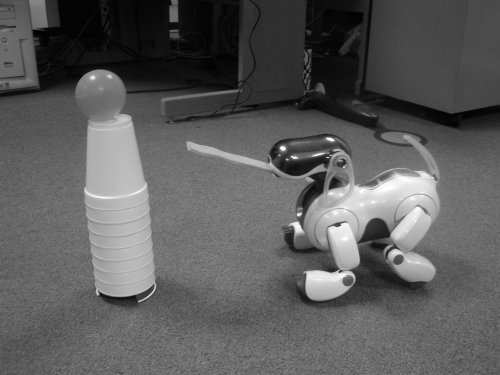
\includegraphics[width=0.45\textwidth]{wood-aibo1} } \quad
%
\subfloat
{ 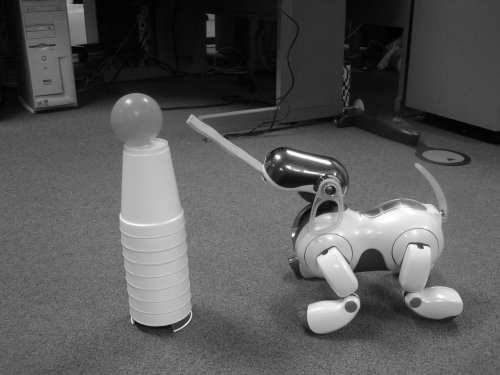
\includegraphics[width=0.45\textwidth]{wood-aibo2} }
\caption{Sequence of frames of a robot using a stick tool, reproduced from~\cite{wood:2005:sieds}.}
\label{fig:tool:wood-aibo}
\end{figure}

One of the first examples of a robot computational model designed to acquire tool use capabilities is~\cite{wood:2005:sieds}.
In this work, a Sony Aibo dog-like robot is equipped with an artificial neural network to learn appropriate postures for grasping a stick tool and thus for reaching a faraway ball on a tower, as shown in Fig.~\ref{fig:tool:wood-aibo}.
Implicitly, it is relying on an internal representation of its body (a body schema) with the attached tool: we will elaborate on this concept for visually processing images of robot hands in Sec.~\ref{sec:tool:approach:hand_to_tool}.

\begin{figure}
\centering
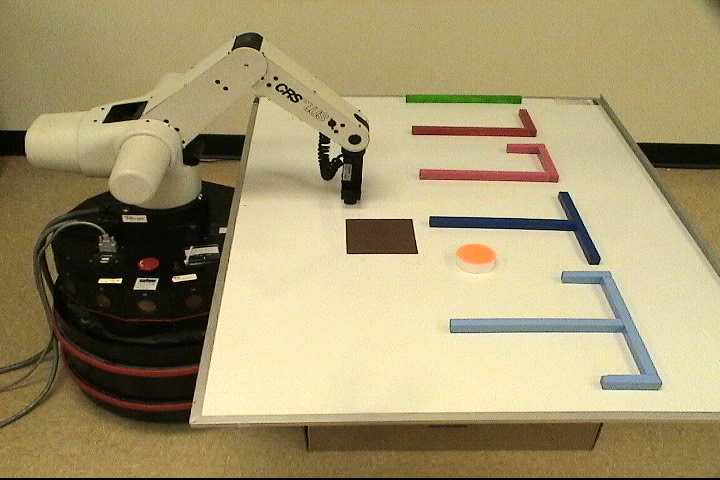
\includegraphics[width=0.7\textwidth]{stoytchev-setup}
\caption{A robot arm with different tools and an orange target object, reproduced from~\cite{stoytchev:2008:lnai}.}
\label{fig:tool:stoytchev-setup}
\end{figure}

The works by Stoytchev and Sinapov \cite{stoytchev:2005:icra,sinapov:2007:icdl,stoytchev:2008:lnai} propose to learn tool affordances as
\toolbehavior{} pairs which yield a desired effect on a robot manipulator, shown in Fig.~\ref{fig:tool:stoytchev-setup}.
Using a number of possible tools (designed to be similar to the ones used by~\cite{kohler:mentality_of_apes} in experiments with chimpanzees), the robot arm explores different possible behaviors and observes their effects on the environment.
We should note that these models learn the affordances of specific tools (i.e., considered as individual entities), however no association between the distinctive features of a tool and its affordances is made.
Therefore, the generalization capabilities of these models are limited to dealing with smaller and larger versions of known tools.

Tikhanoff \cite{tikhanoff:2013:humanoids} focuses on an iCub robot learning the specific tool affordance of pulling.
This is done by learning a relationship between angles of the robot action being exerted, and distance traveled by objects on the table, after a series of pull actions.
Although useful for robot operations, this knowledge is specific for the tool that is experienced at training time, and it cannot be easily generalized to novel, previously unseen, tools.
This limitation is relaxed by Mar \cite{mar:2018:tcds}: visual features are extracted from the functional part of the tool (also accounting for the way in which the tool is grasped), and they are related to the effects observed after the robot action.
This allows to robustly adjust the motion parameters depending on how the tool is grasped by the robot.
However, the target object's shape is not taken into consideration and, as such, the influence of the object on the measured effects is not studied.
In addition, that system starts with the tool in the robot's hand: therefore, it does not address tool selection.

In~\cite{jain:2013:alr}, a \ac{BN} is used to model tool affordances as probabilistic dependencies between actions, tools and effects.
To address the problem of predicting the effects of unknown tools (i.e., the generalization ability of the model), the authors of that work propose a tool representation based on the functional features of the tool (geometrical features, e.g., corners, bars, etc.), arguing that those features can remain distinctive and invariant across different tools used for performing similar tasks.
However, it is not clear how those features are computed or estimated, if they can be directly obtained through robot vision and if they can be applied to different classes of tools.
Also, the functional features in that system have to be annotated by hand, contrary to other works such as~\cite{mar:2018:tcds}.

It is worth noting that in
\cite{stoytchev:2005:icra,sinapov:2007:icdl,stoytchev:2008:lnai,tikhanoff:2013:humanoids,mar:2018:tcds,jain:2013:alr}
the properties
of the acted objects are not explicitly considered in the model;
only the general affordances of tools are learned, regardless
of the objects that the tools act upon.
Instead, in our model we relate the properties of the acted objects with the properties of the tools.

Abelha and Guerin \cite{abelha:2017:iros} propose a system that, given a specified task and some available candidate tools in a scene, learns to predict the individual tool affordances (the results are in the form of pixelwise scores, as well as the regions for grasping and using tools).
Prior task knowledge is learned from simulating actions with~116 object CAD models available from the web.
One strength of this system is that, in addition to predicting how well a tool part affords a task, it also provides geometric manipulation cues (indicating the region for grasping the tool and the region for using it onto the target object), thus exploring the idea that a tool potentially possesses many ways in which it can be used for a given task.
However, this work is done in simulation only: not only is it not evaluated on a real robot, but even these simulations are not embodied in any specific robot.
Because of this limitation and of the differences between all the end effectors that exist in real robots, the applicability of such a work on real robots remains to be seen.

Moldovan and colleagues consider a multi-object scenario \cite{moldovan:2018:ar} in which the relational affordances between objects pairs are exploited to \emph{plan} a sequence of actions to achieve a desired goal, using probabilistic reasoning (we will elaborate on the usefulness of affordances for planning in Ch.~\ref{chap:poeticon++_case_study}).
The pairwise interactions are described in terms of the objects' relative distance, orientation and contact.
However, the authors of that work do not investigate how these interactions are affected by different geometrical properties of the objects.

In Sec.~\ref{sec:tool:related_work:psychology} we analyzed the possible link from hand affordances to tool affordances.
To the best of our knowledge, ours is the first contribution, in the robot affordances field, which explicitly looks at the visuomotor possibilities offered by different hand morphologies and postures~(e.g., hands with straight fingers, bent fingers, or arched fingers, see Fig.~\ref{fig:robot_hand_postures}).
We exploit this information to acquire, through self-exploration, a model that is able to generalize to novel situations for a robotic agent, including making the crucial developmental leap from hand use to tool use, as observed in babies by psychology studies.

%%%%%%%%%%%%%%%%%%%%%%%%%%%%%%%%%%%%%%%%%%%%%%%%%%%%%%%%%%%%%%%%%%%%%%%%%%%%%%%%
\section{Proposed Approach}
\label{sec:tool:approach}

Fig.~\ref{fig:tool:tools_computational_model} shows a diagram of our computational model of affordances for dealing with multiple objects and, thus, permitting tool use behavior.
Our model is an extension of the model by Montesano (see \cite{montesano:2008} and Sec.~\ref{sec:background:previous_works:montesano}), which had the limitation of the robotic agent dealing with one object only.
By contrast, our extension permits the agent to consider a pair of entities: a manipulator (i.e., the held object in the robot's hand, or the bare hand itself) and an acted object upon which actions are executed.

Below, we describe our proposed approach as follows.
Sec.~\ref{sec:tool:approach:model} illustrates the reasoning model of \intobj{} affordances.
In Sec.~\ref{sec:tool:approach:learning} we show how to learn affordances of multiple objects and tools, including the transfer of knowledge from simulation to a real robot.
Finally, in Sec.~\ref{sec:tool:approach:hand_to_tool} we explore the developmental link from hand affordances to tool affordances.

Notably, in Sec.~\ref{sec:tool:approach:learning} (\cite{goncalves:2014:icdl}) the concept of toolness is not specified in the model, but it emerges from experiments.
Instead, in Sec.~\ref{sec:tool:approach:hand_to_tool} (\cite{saponaro:2017:icdl}) the concept of toolness is a starting hypothesis, and the focus is on the developmental transition from hand to tool affordances.

%%%%%%%%%%%%%%%%%%%%%%%%%%%%%%%%%%%%%%%%%%%%%%%%%%%%%%%%%%%%%%%%%%%%%%%%%%%%%%%%
\subsection{Computational Model}
\label{sec:tool:approach:model}

The computational formulation of affordances by Montesano \cite{montesano:2008} models affordances as \actobjeff{} triplets (see Sec.~\ref{sec:background:previous_works:montesano}).
Due to this formulation, only certain robot scenarios can be considered: those where the action is applied to a \emph{single object} using the robot hands and the effects are observed.
In this section, we extend that formulation by explicitly modeling both the manipulator (e.g., the held object) and the acted object (i.e., the target of the action) with corresponding variables\footnote{For now, we consider the manipulator node of Fig.~\ref{fig:tool:tools_computational_model} to refer to the held object (i.e., tool). Later on in the chapter, we will consider the special case when this manipulator is the robot's bare hand.}, thus reasoning about \emph{\intobj} affordances.
We do this by modifying the visual affordance and reasoning framework of Sec.~\ref{sec:platform:software_architecture}.

We now illustrate our model to capture meaningful relationships between actions, effects, manipulators and acted objects.

\begin{figure}
\centering
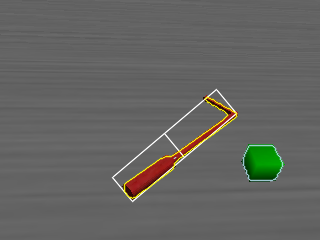
\includegraphics[width=0.5\textwidth]{tool_seg_simulator_ICARSC}
\caption[Two environment objects being visually processed in simulation.]%
{Two environment objects being visually processed in simulation.

Left: a possible manipulator (held object or tool), whose segmented silhouette is divided in two parts (top and bottom) along its main axis.

Right: possible acted object.
This one is also divided in two parts by the model, however we do not show the halves graphically when the whole object's compactness descriptor is above an empirically-defined threshold (which only affects the display, not the experiments).

From each object and each object part we compute a set of shape descriptors, used to build the tool affordances knowledge.
Compare with Fig.~\ref{fig:shape_features_pipeline} on p.~\pageref{fig:shape_features_pipeline} for the one-object case.}
\label{fig:tool+object_segmentation_example}
\end{figure}

Both the manipulator and the acted object are represented by
the pre-categorical shape descriptors (described in Sec.~\ref{sec:platform:software_architecture:visual_pipeline}) of visually segmented objects (``blobs'') seen by the robot.
The shape descriptors employed here are a subset of the ones reported in Table~\ref{tab:descriptors} on p.~\pageref{tab:descriptors}: convexity, eccentricity, compactness, circularity, squareness.

The most distinctive aspect of our model with respect to the state of the art is that we consider elongated objects split in two halves along its main axis, as shown in the example of Fig.~\ref{fig:tool+object_segmentation_example}.

The intuition for reasoning about sub-parts (halves) of tools is that the affordance offered by a tool often resides in only the most salient and functional part of the tool perceived by the agent~\cite{lockman:2000:childdev}, not in the entirety of it.
A hammer tool affords the action of hitting a nail so that it enters a wall, and this capability resides in the characteristics of the tip of the hammer~(e.g., the shape and the material of the tip).

For reasoning on tool affordances with robot perception algorithms, the graphical splitting of a tool along its main axis is a simple yet helpful way to capture affordances of manipulator (held) objects, for which only the effector part (tip part, or non-grasped part) physically interacts with the acted object.
Note that, when the robot sees a possible manipulator object lying on the table, in our model any of the two halves could be potentially used as effector: \emph{we do not pre-program which of the halves is the handle and which is the effector}, but we let the robot discover that by \emph{autonomous exploration}, following the developmental robotics perspective described in Sec.~\ref{sec:motivation:devrob}.

For manipulators (held objects), the \acl{BN} variables that we consider are the visual descriptors of one of the object halves: during learning, the half that is not grasped is considered; during inference (e.g., effect prediction, tool selection, action selection), each of the halves can be considered, if the held object has not been grasped yet.
For acted objects, the whole blob visual descriptors are used (i.e., the blob is not split in two halves).
As in p.~\pageref{para:objects}, each shape descriptor has a value that can range within three empirically-defined discrete levels.

In terms of motor \emph{actions} performed by the agent with a manipulator (held) object in its hand onto an acted object on the table, we consider the following pre-defined directional movements:
left lateral tap,
right lateral tap,
pull closer,
push away.

The discrete identifiers of these four actions are the values of the action node in the affordance \acp{BN}.

\begin{figure}
\centering
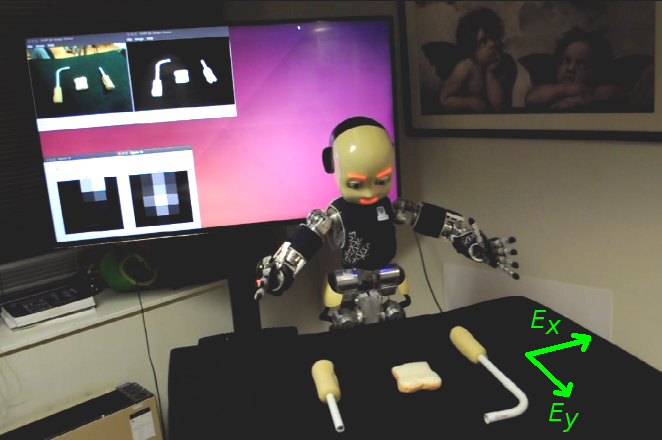
\includegraphics[width=0.4\linewidth, clip, trim=8.5cm 0cm 2cm 0cm]{iCub_selecting_between_two_tools2}
\caption{The iCub robot in a tool use scenario, with green overlay arrows showing the effects (i.e., displacements of objects).}
\label{fig:iCub_selecting_between_two_tools_green_overlays}
\end{figure}

Finally, as for the resulting \emph{effects}, we do as in p.~\pageref{para:effects} in terms of modeling the two directions of displacement (lateral and longitudinal) of the acted object on a tabletop, each direction having a value that can range within five empirically-defined discrete levels of possible displacement magnitude.
Fig.~\ref{fig:iCub_selecting_between_two_tools_green_overlays} shows an illustration, with the two effects marked~$E_x$ and~$E_y$.

Our model allows to predict the motion effects induced by the motor action being exerted by the robot and the shape descriptors of the two objects involved:
$p(\EffectX, \EffectY \given A, T, O)$,
where~$\EffectX$ is the lateral motion of the acted object on the table,
$\EffectY$ is its longitudinal motion,
$A$ is an identifier of the robot action~(e.g., pushing, pulling),
$T$ is the vector of shape descriptors of the manipulator (tool) held in the robot's hand, and
$O$ is the vector of shape descriptors of the acted object on the table.

%%%%%%%%%%%%%%%%%%%%%%%%%%%%%%%%%%%%%%%%%%%%%%%%%%%%%%%%%%%%%%%%%%%%%%%%%%%%%%%%
\subsection{Learning}
\label{sec:tool:approach:learning}

In this section, we show how to learn from data our computational model for tool use affordances described in Sec.~\ref{sec:tool:approach:model}.
We compare different \aclp{BN} that implement our model, to determine the most suitable one.
The comparison is in terms of memory complexity, prediction ability and generalization capability.
In all the \acl{BN} structures that we discuss, we use discrete variables and \ac{MAP} probability estimates to learn the \ac{CPD} table parameters.

To begin with, we capture these relationships \emph{in simulation}, which has the advantage of letting us run hundreds of robot manipulation experiments without the cost associated to real robot experiments.
Later, we will see how it is possible to transfer tool use affordances knowledge from a simulated robot to a real robot, making predictions in the real world, and take optimal decisions with respect to a desired outcome during manipulation.

\begin{figure}
\centering
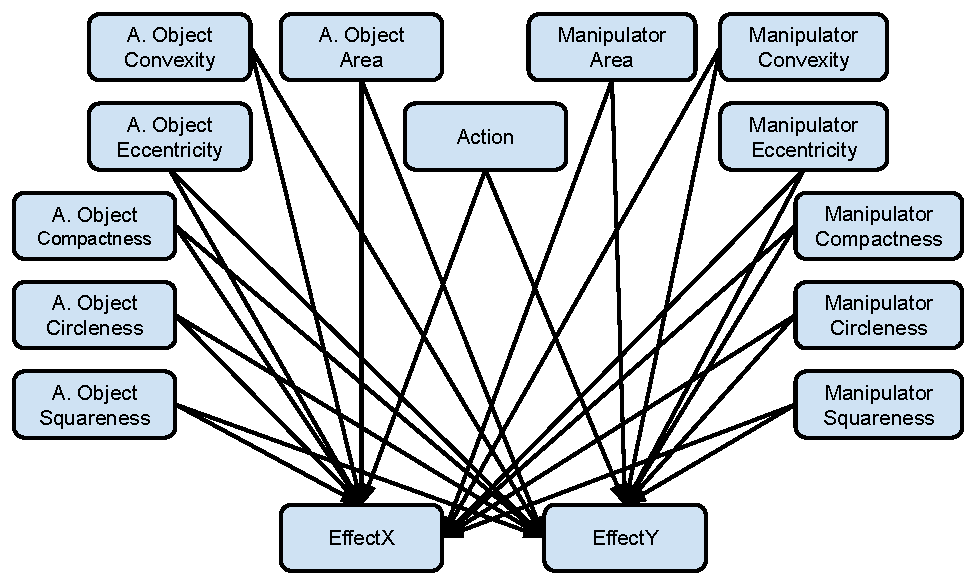
\includegraphics[width=0.9\textwidth]{tool_nets_full}
% footnote within caption, https://tex.stackexchange.com/a/67030
\caption[Fully connected \acl{BN} structure to encode \intobj{} affordances.]{Fully connected \acl{BN} structure to encode \intobj{} affordances.
A.~Object means Acted Object, Manipulator refers to the held object.
This structure was specified manually.}
\label{fig:tool:nets:full}
\end{figure}

\begin{figure} % contains a figure and a table on the same page, https://tex.stackexchange.com/a/111121
\centering
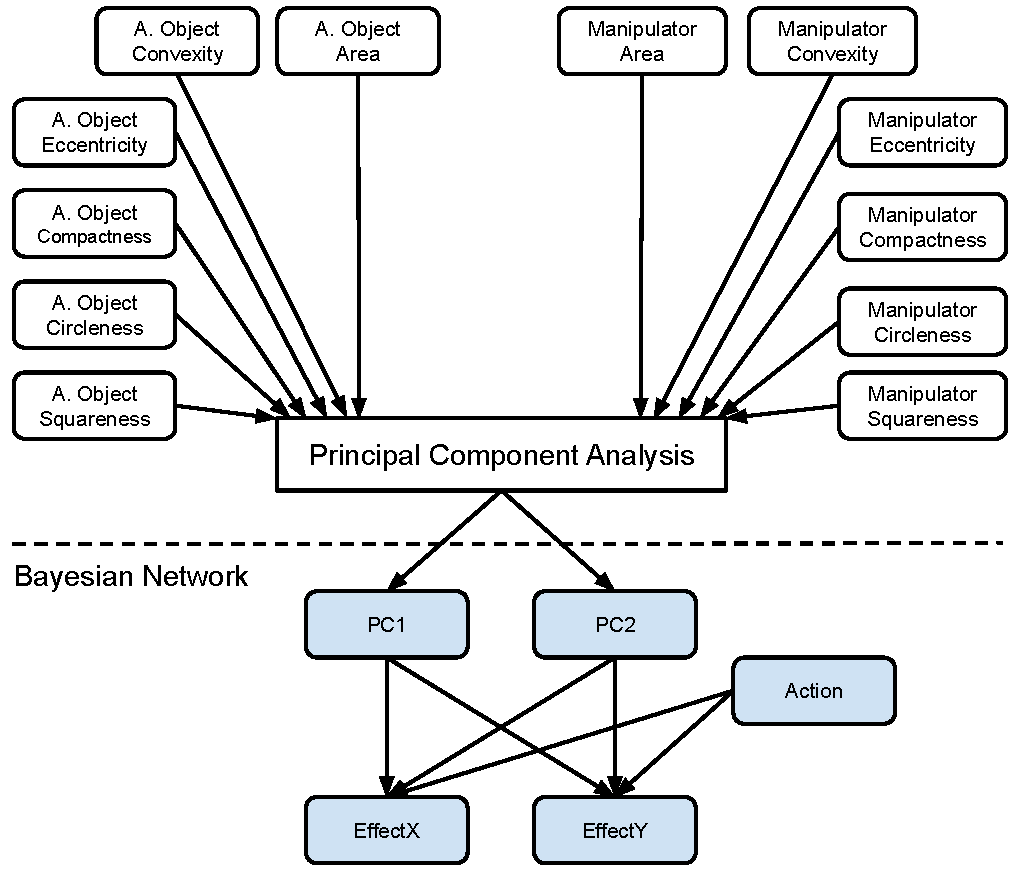
\includegraphics[width=0.9\textwidth]{tool_nets_pca2014}
\caption[Dimensionality-reduced \acl{BN} structure to encode \intobj{} affordances, adapted from \cite{goncalves:2014:icdl}.]{Dimensionality-reduced \acl{BN} structure to encode \intobj{} affordances, adapted from \cite{goncalves:2014:icdl}.
A.~Object means Acted Object, Manipulator refers to the held object.
This structure was specified manually, after having empirically tried different \ac{PCA} hyper-parameters, see Table~\ref{tab:tool:tool_pca_hyperparams}.
The \ac{PCA} dimensionality reduction is computed on the continuous vectors of the visual features.

In this case, there is one \ac{PCA} block for the whole original visual feature space with~12 dimensions (6 features for the manipulator or held object, and~6 for the acted object, considered jointly).
This is because the concept of toolness was not specified in this work, but was emerging from experiments.}
\label{fig:tool:nets:pca2014}
%
\captionof{table}[Hyper-parameters used to train the \acl{BN} of Fig.~\ref{fig:tool:nets:pca2014}.]{%
Hyper-parameters used to train the \acl{BN} of Fig.~\ref{fig:tool:nets:pca2014} for predicting the distribution of the effects.
} % end captionof
    \scriptsize
    \begin{tabular}{*{2}{l}} % left-aligned columns
    \toprule
    parameter & value (and comment) \\
    \midrule
    number of \acs{PCA} blocks                   & $1$ (manipulator and acted object features considered jointly) \\
    number of components in the \acs{PCA}        & $2$ \\
    number of discretization values (bins)       & $3$ \\
    of each \acs{PCA} component                  & \\
                                                 & \\
    number of discretization values (bins)       & $5$ \\
    of each $\Effect$ node                       & \\
                                                 & \\
    intervals (in meters) of the $\Effect$ bins  & $\interval[open left]{-\infty}{-0.06}$, $\interval[open left]{-0.06}{-0.025}$, \\
                                                 & $\interval[open left]{-0.025}{0.025}$, $\interval[open left]{0.025}{0.06}$, $\interval[open]{0.06}{\infty}$ \\
    \bottomrule
    \end{tabular}
    \label{tab:tool:tool_pca_hyperparams}
\end{figure}

\begin{figure}
\centering
\subfloat[][K2 \StructureLearning{} network.]
{ 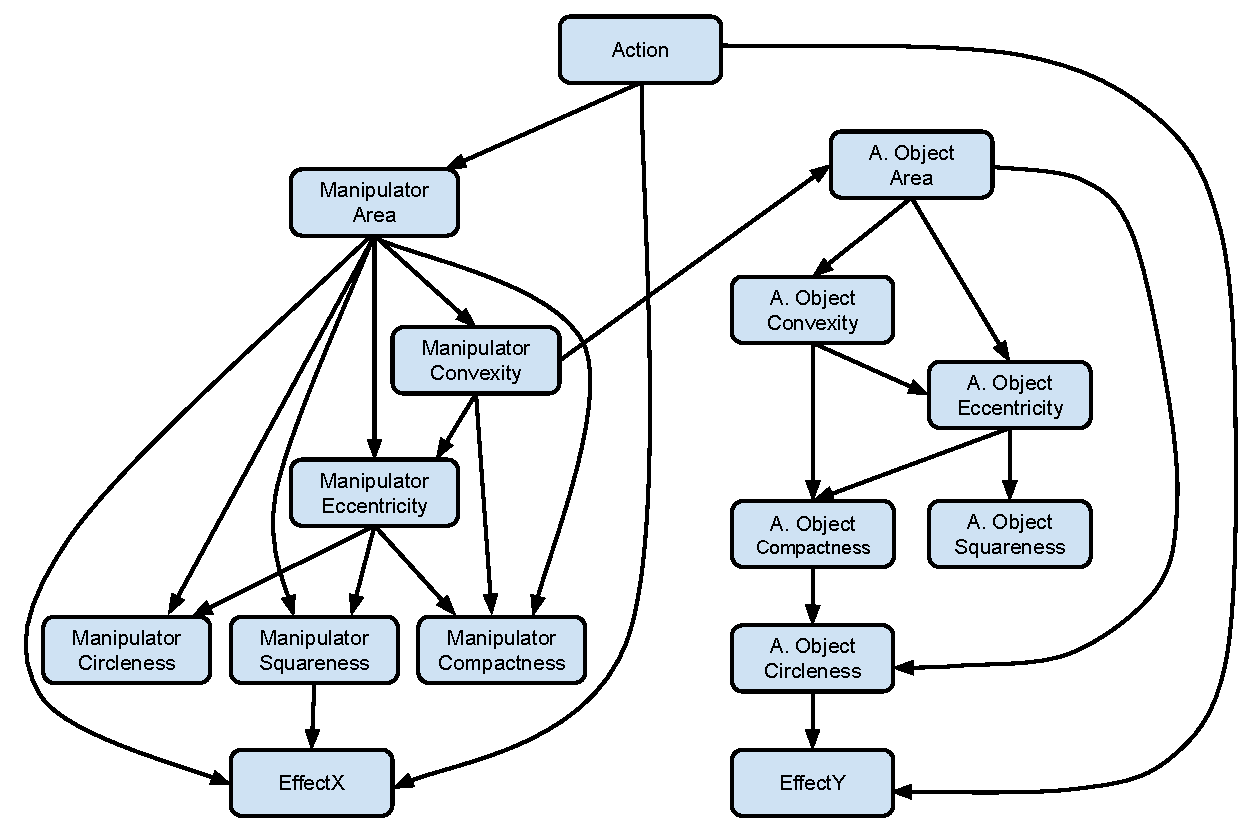
\includegraphics[width=0.9\textwidth]{tool_nets_k2} \label{fig:tool:nets:k2} } \\
%
\subfloat[][BDe \StructureLearning{} network.]
{ 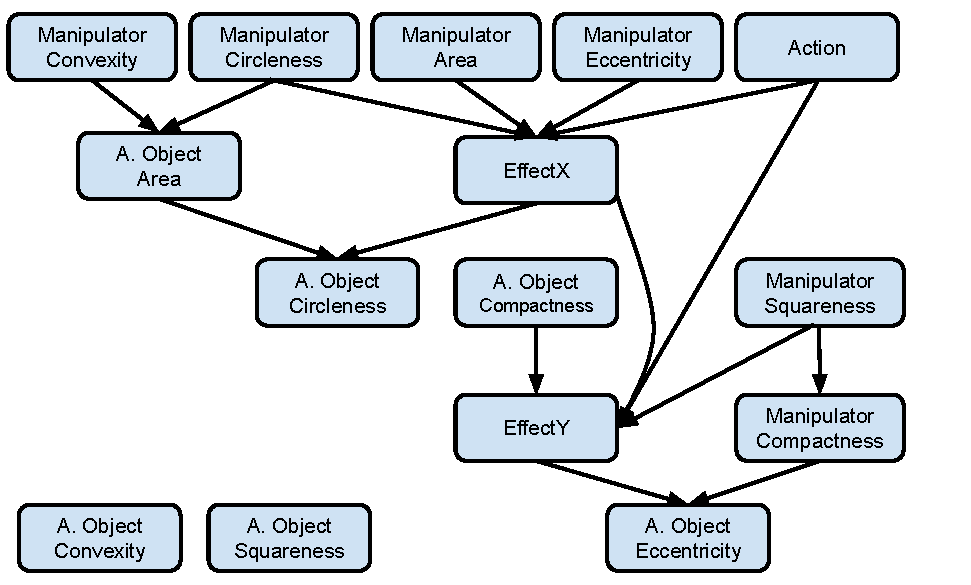
\includegraphics[width=0.9\textwidth]{tool_nets_bde} \label{fig:tool:nets:bde} }
\caption[\StructureLearning{} \acl{BN} structures to encode \intobj{} affordances.]{\StructureLearning{} \acl{BN} structures to encode \intobj{} affordances.
A.~Object means Acted Object, Manipulator refers to the held object.
These structures were obtained from experimental data.}
\label{fig:tool:nets:structure_learning}
\end{figure}

The first, baseline structure for our comparisons is a manually defined \emph{fully connected} network, shown in Fig.~\ref{fig:tool:nets:full}.
This is the most general structure, in which all the acted object, manipulator (held object) and action nodes are connected to the effect nodes.

The fully connected network suffers from a number of limitations: low performance, overfitting, large number of parameters.
Basically, this network structure suffers from the curse of dimensionality\footnote{%
The curse of dimensionality \cite[p.~33]{bishop:prml} is a difficulty arising when we add more features to a pattern recognition model (i.e., when we increase the dimensionality of its feature space), which in turn requires to collect more data. The amount of data that we need to collect to avoid overfitting grows exponentially as we add more dimensions.}. % end footnote
Each effect node has a high number of parents.
In our case~6 for the manipulator (held object), plus~6 for the acted object, plus~1 for the action, in total~13: this results in big \ac{CPD} tables, which makes the network hard to train and unfit to generalize the trained observations to unseen situations.

The second structure is a dimensionality-reduced one.
To reduce the dimensionality of the feature space, we apply \acf{PCA}\footnote{%
\ac{PCA} is a technique for dimensionality reduction and feature extraction.
It attempts to find a (linear) sub-space of lower dimensionality than the original input space, where the new features have the largest variance \cite[p.~561]{bishop:prml}.% end footnote
} to the features seen in our training data, as shown in the upper part of Fig.~\ref{fig:tool:nets:pca2014} in white.
We use~$80\%$ of our experimental data for training and~$20\%$ for testing,
where the original feature space has~12 dimensions:
6 features for the manipulator (held object) and~6 for the acted object, considered jointly.

\ac{PCA} provides the~12 eigenvectors and eigenvalues computed from the data matrix, of which, however, we only need the~2 Principal Components with the highest significance (i.e., the~2 with the highest eigenvalue), to explain over~$99\%$ of the data variance.
This shows that acted object and manipulator features are highly correlated.
Therefore, we create two nodes, each corresponding to a Principal Component, and these, along with the action node, are now the parents of the effect nodes of a \emph{reduced} \acl{BN}, displayed in the lower part of Fig.~\ref{fig:tool:nets:pca2014} in blue.
The values of these nodes are the coefficients of each eigenvector given the observable features.
These coefficients are then discretized, based on the training data, into two bins
(half the data to each bin).
The \ac{PCA} dimensionality reduction is computed on the continuous vectors of the visual features.
This structure was specified manually, after having empirically tried different \ac{PCA} hyper-parameters.
We tried to discretize each node into more bins, but the performance of the network when predicting effects of unseen data got significantly worse.

In Sec.~\ref{sec:background:theory:structure_learning} we have introduced \acl{BN} \StructureLearning{}, that is, the problem of learning the structure of the \ac{DAG} from data, and two common heuristic-based approaches for this problem: K2 and BDe.
We employ these two approaches and compare the performance of the resulting networks (Figs.~\ref{fig:tool:nets:k2} and~\ref{fig:tool:nets:bde}, respectively) with those of the fully connected network and of the \ac{PCA} one.

We use~$80\%$ of our experimental data for training and~$20\%$ for testing.
All the nodes except for $\EffectX$ and $\EffectY$ are entered as interventional variables, defined on p.~\pageref{para:interventional_vars}, which means that we force a node to take a specific value, thereby effectively severing its incoming arcs~\cite{murphy:2012:mlprob}.

The effect prediction inference performed on the networks is of the type $p(\Effect \given \parents(\Effect))$, which, considering for example the topology of the network from Fig.~\ref{fig:tool:nets:pca2014}, amounts to this marginalization over our two effect nodes (horizontal and vertical displacement of the object):
\begin{equation} \label{eq:effect_query}
    p(\EffectX, \EffectY \given M, O, A),
\end{equation}
where $M$~is the vector of features of the manipulator, $O$~is the vector of features of the acted object, $A$~is the motor action identifier.

The measure of \emph{complexity} in Table~\ref{tab:tool:complexity} is computed as the number of elements in the largest \ac{CPD} of a network.
Complexity depends only on the discretization and on the network structure, independently of data and learning.

\begin{table}
\caption[Complexity of affordances \aclp{BN}.]{Complexity of affordances \aclp{BN}, computed as the sum of the elements in the \acp{CPD} of all nodes.}
\label{tab:tool:complexity}
\centering
\begin{tabular}{*{4}{p{0.15\columnwidth}}} % four p{} columns
\toprule
Baseline   & \acs{PCA}   & \StructureLearning{} BDe & \StructureLearning{} K2 \\
\midrule
\num{21257680} & $\bm{168}$ & \num{1594} & $535$ \\
\bottomrule
\end{tabular}
\end{table}

%%%%%%%%%%%%%%%%%%%%%%%%%%%%%%%%%%%%%%%%%%%%%%%%%%%%%%%%%%%%%%%%%%%%%%%%%%%%%%%%
\subsection{Hand to Tool Transition}
\label{sec:tool:approach:hand_to_tool}

\begin{figure}
    \centering
    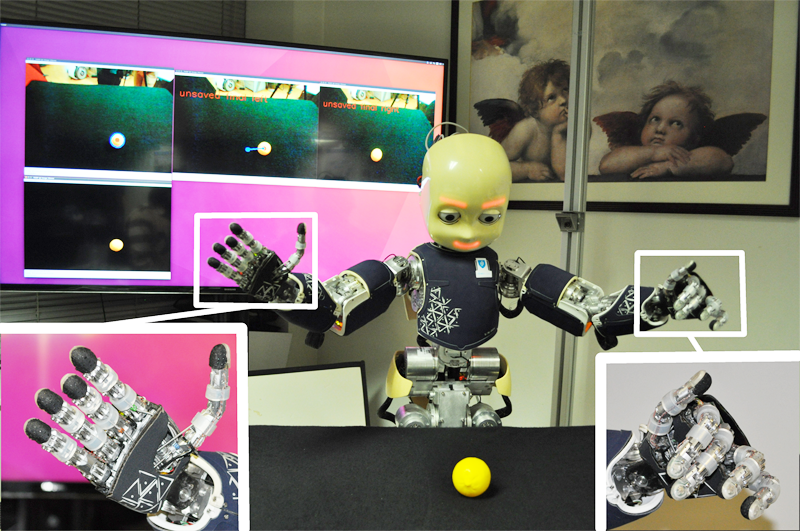
\includegraphics[width=0.9\textwidth]{icub_with_different_hands-smaller2_lighter}
    \caption[The iCub humanoid robot performing motor actions with different hand postures onto a physical object.]{The iCub humanoid robot performing motor actions with different hand postures onto a physical object. In the background screen, we show the visual routines that monitor the evolution of the environment.}
    \label{fig:iCub_with_different_hand_postures}
\end{figure}

We now show how the model presented in the previous sections can be adapted for learning the affordances of different hand postures (e.g., hands with straight fingers, bent fingers, or arched fingers, see Fig.~\ref{fig:robot_hand_postures}).
This approach is useful for implementing the developmental leap from hand use to tool use on a humanoid robot.

One important motivation to study this problem is the \emph{cost of data acquisition}.
While a robot can collect many sensorimotor experiences using its own hands, this cannot happen for all possible human-made tools.
Therefore, we investigate the developmental transition from hand to tool affordances: what sensorimotor skills that a robot has acquired with its bare hands can be employed for tool use?

\begin{figure*}
    \subfloat
    {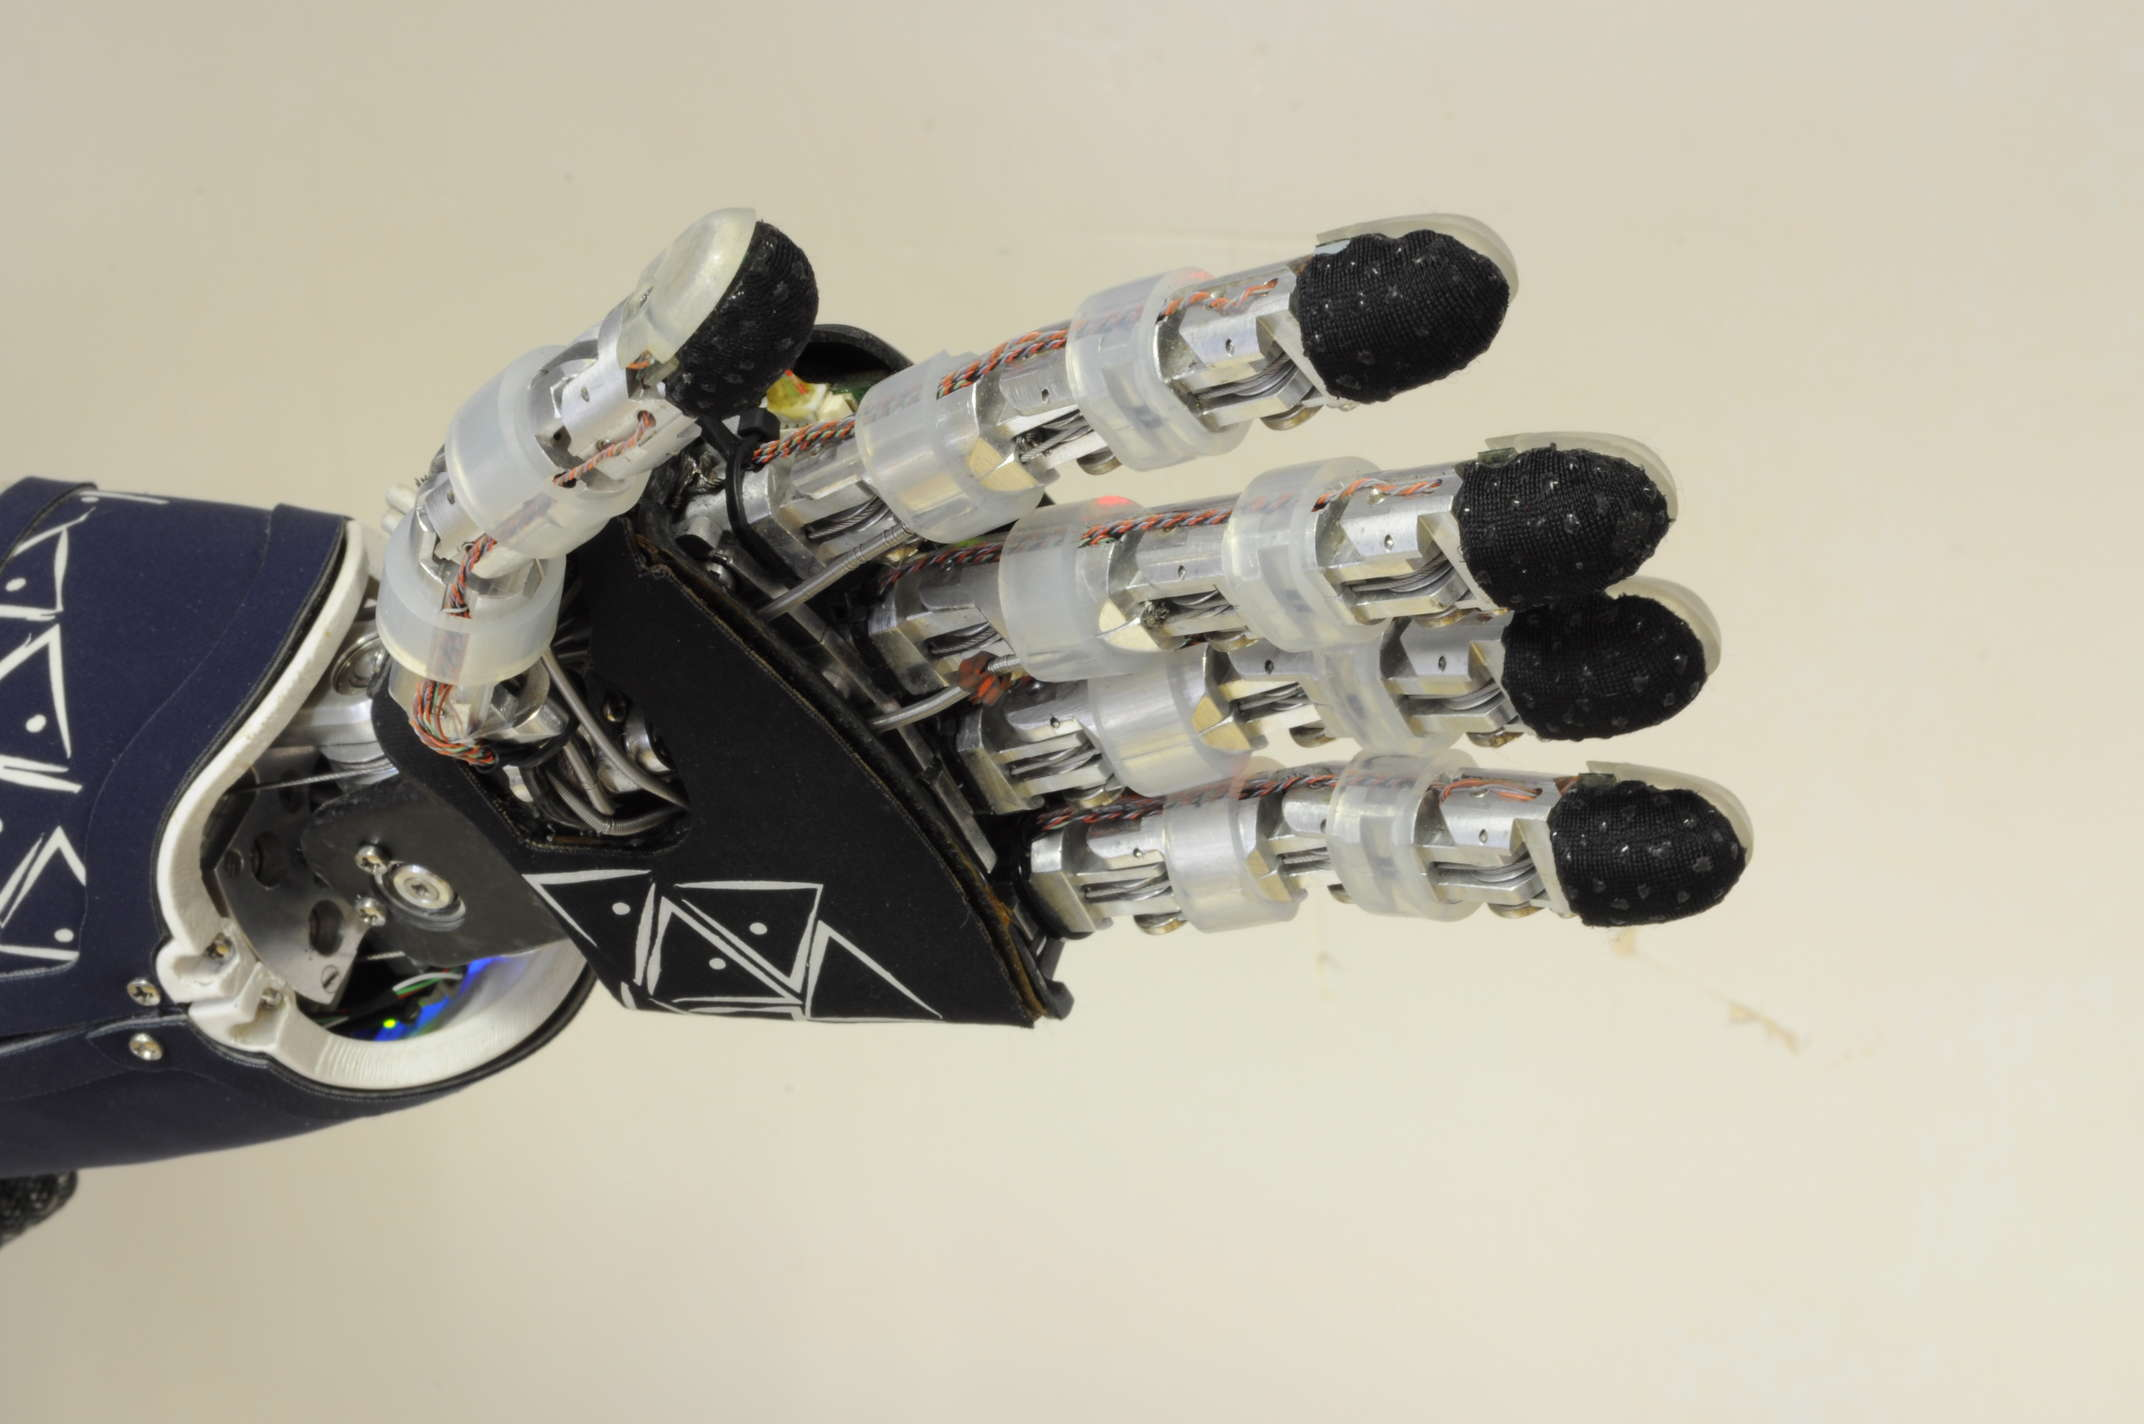
\includegraphics[width=0.3\textwidth]{persp1_straight} } \quad
    %
    \subfloat
    {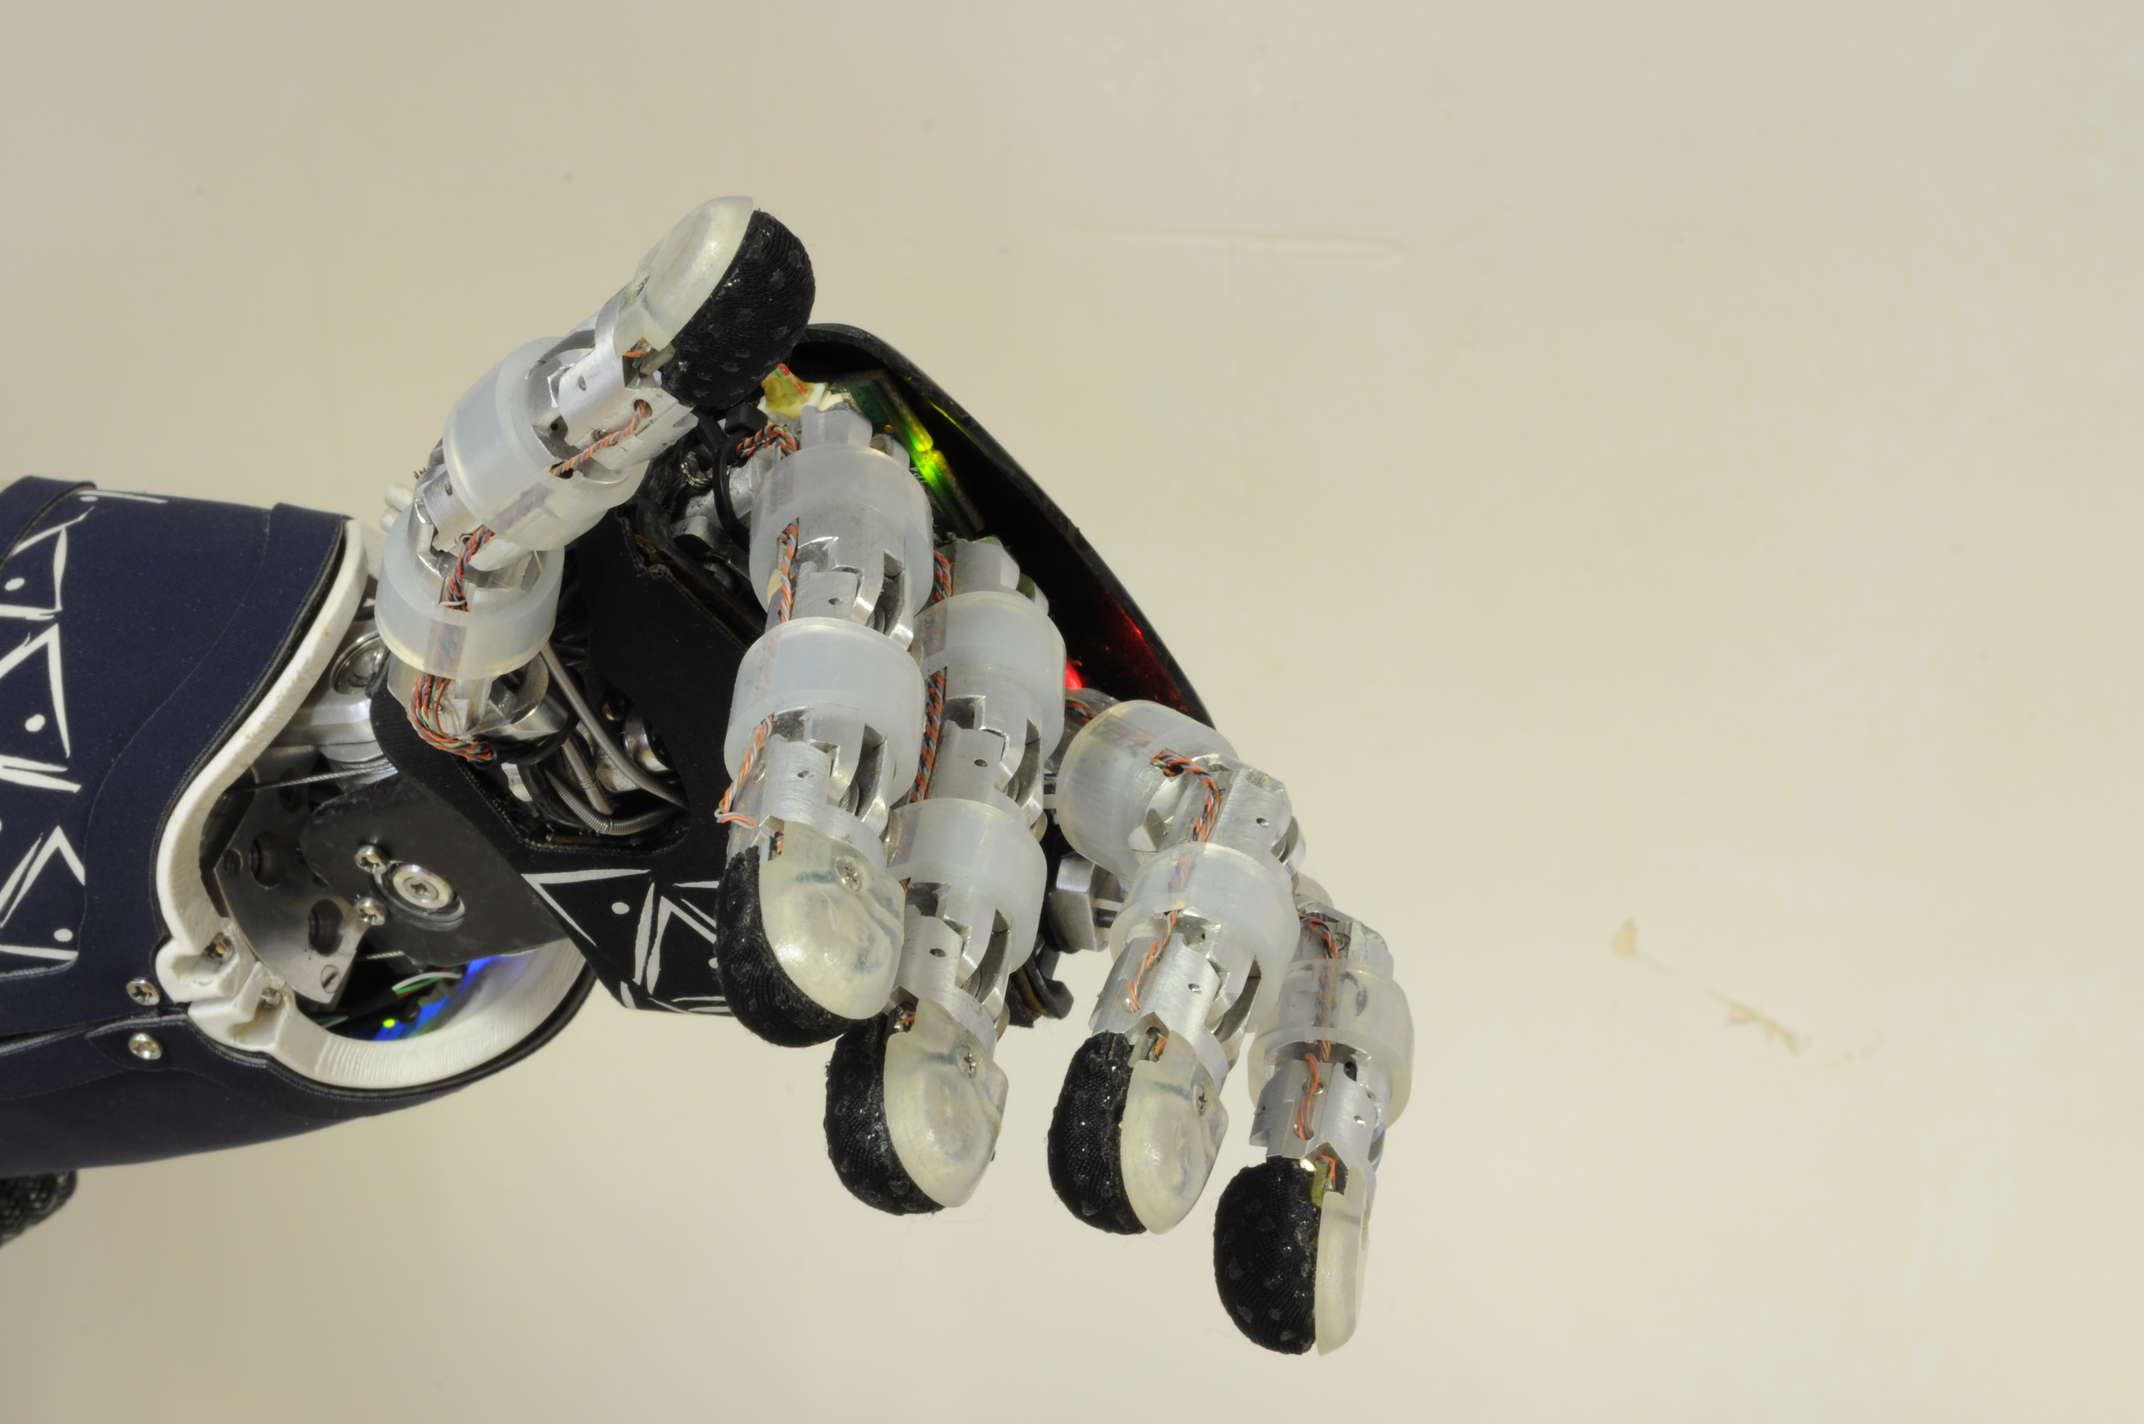
\includegraphics[width=0.3\textwidth]{persp1_bent} } \quad
    %
    \subfloat
    {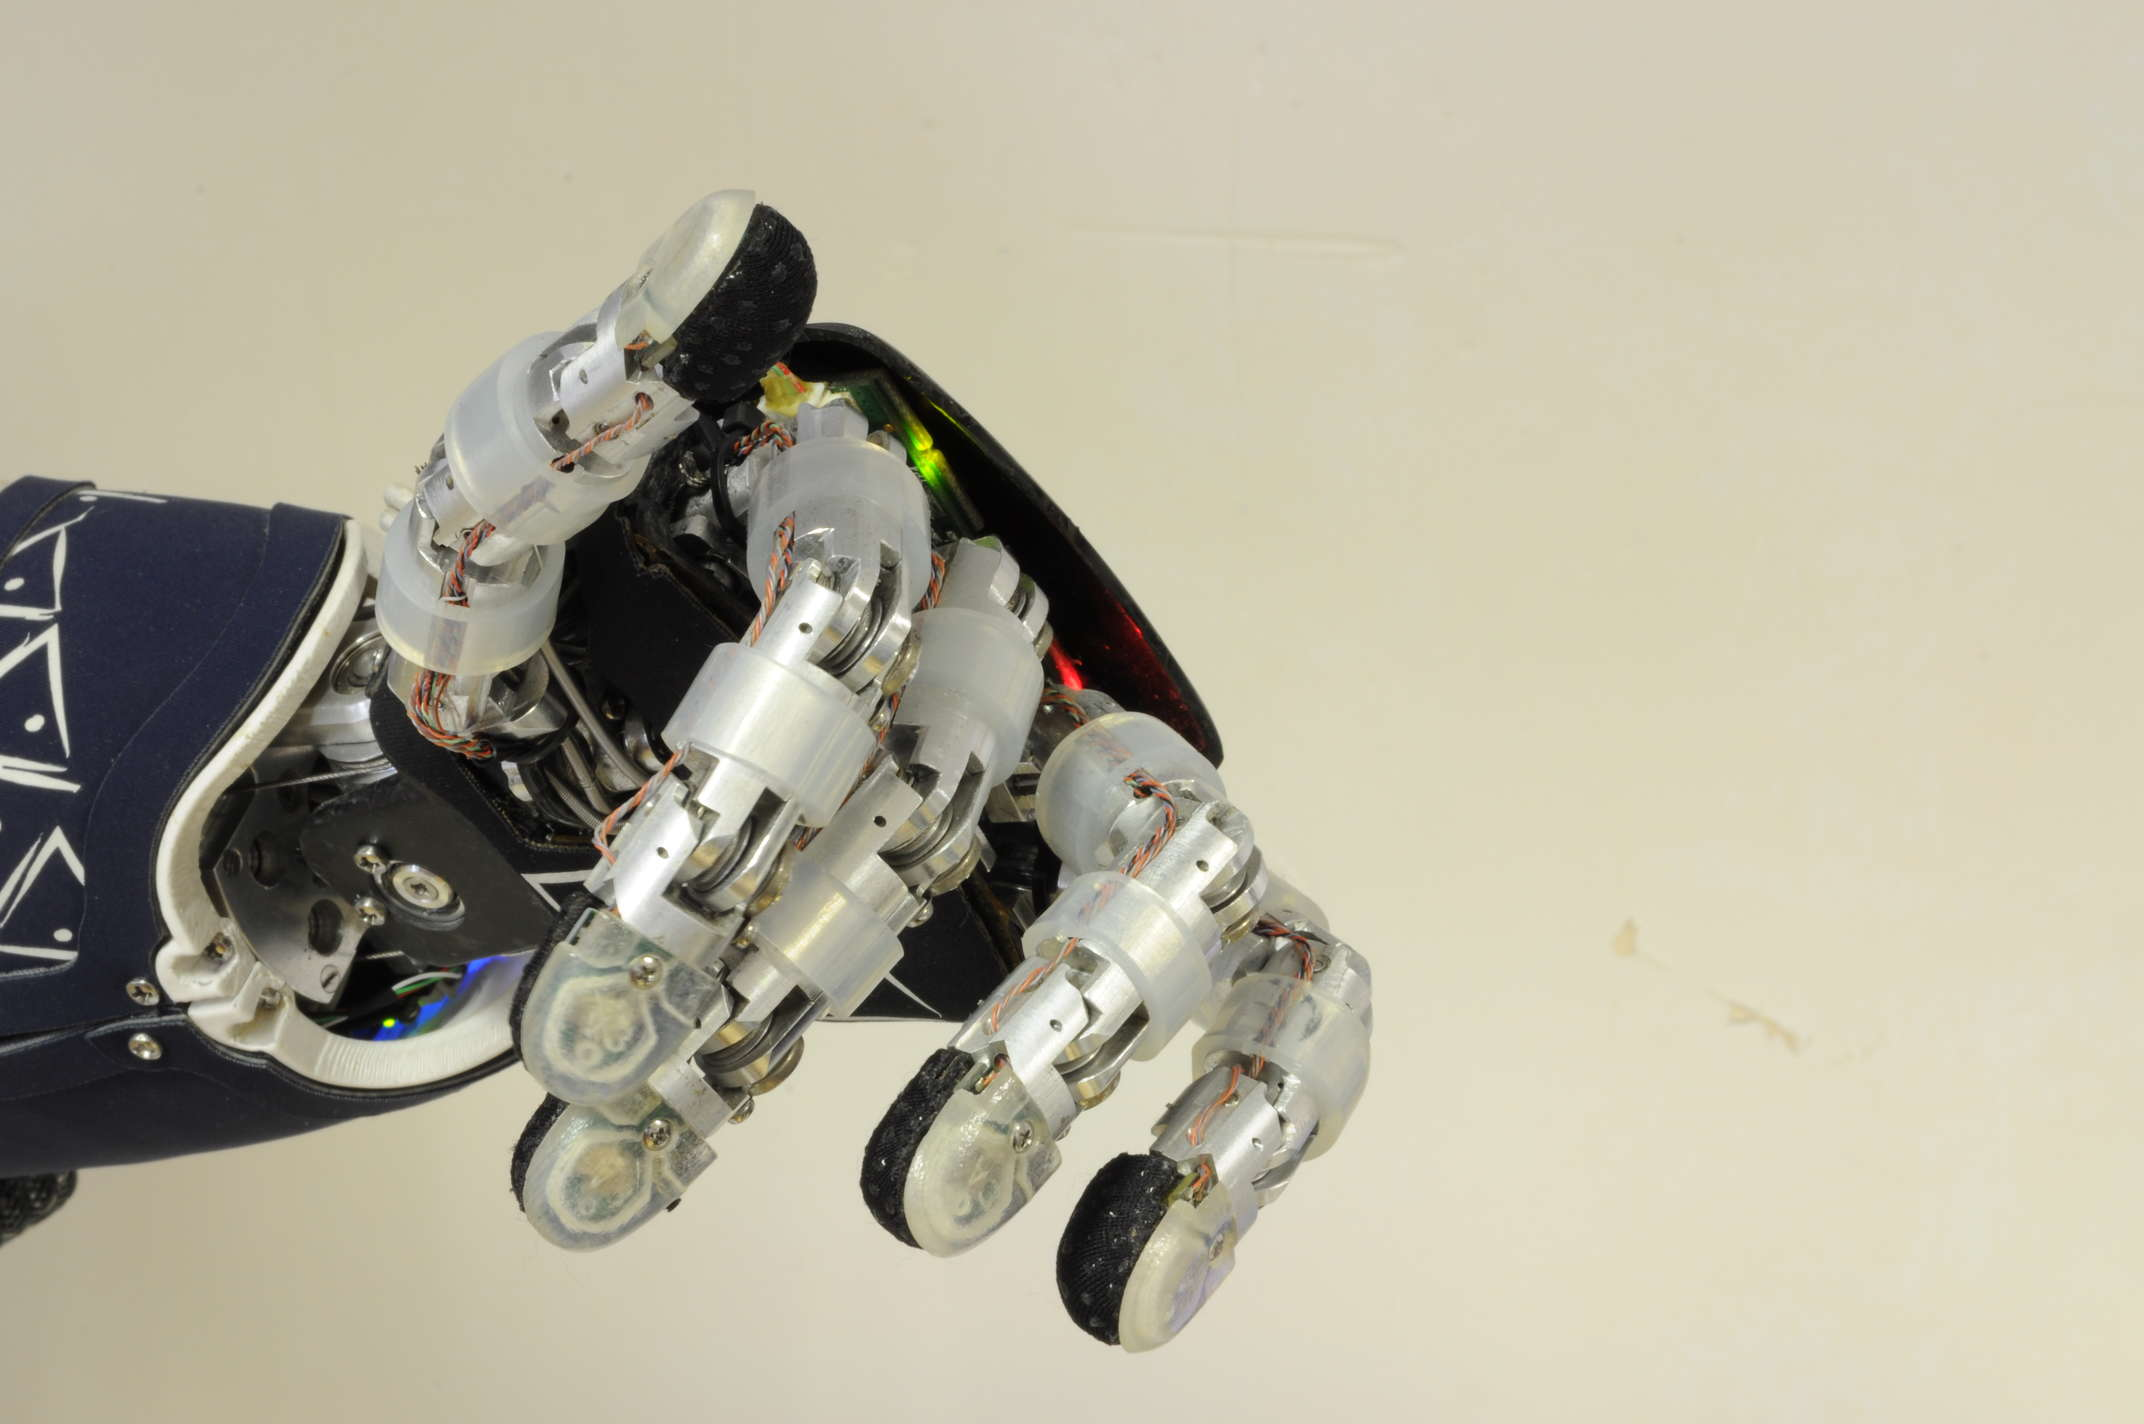
\includegraphics[width=0.3\textwidth]{persp1_fortyfive} } \\
    %
    \subfloat
    {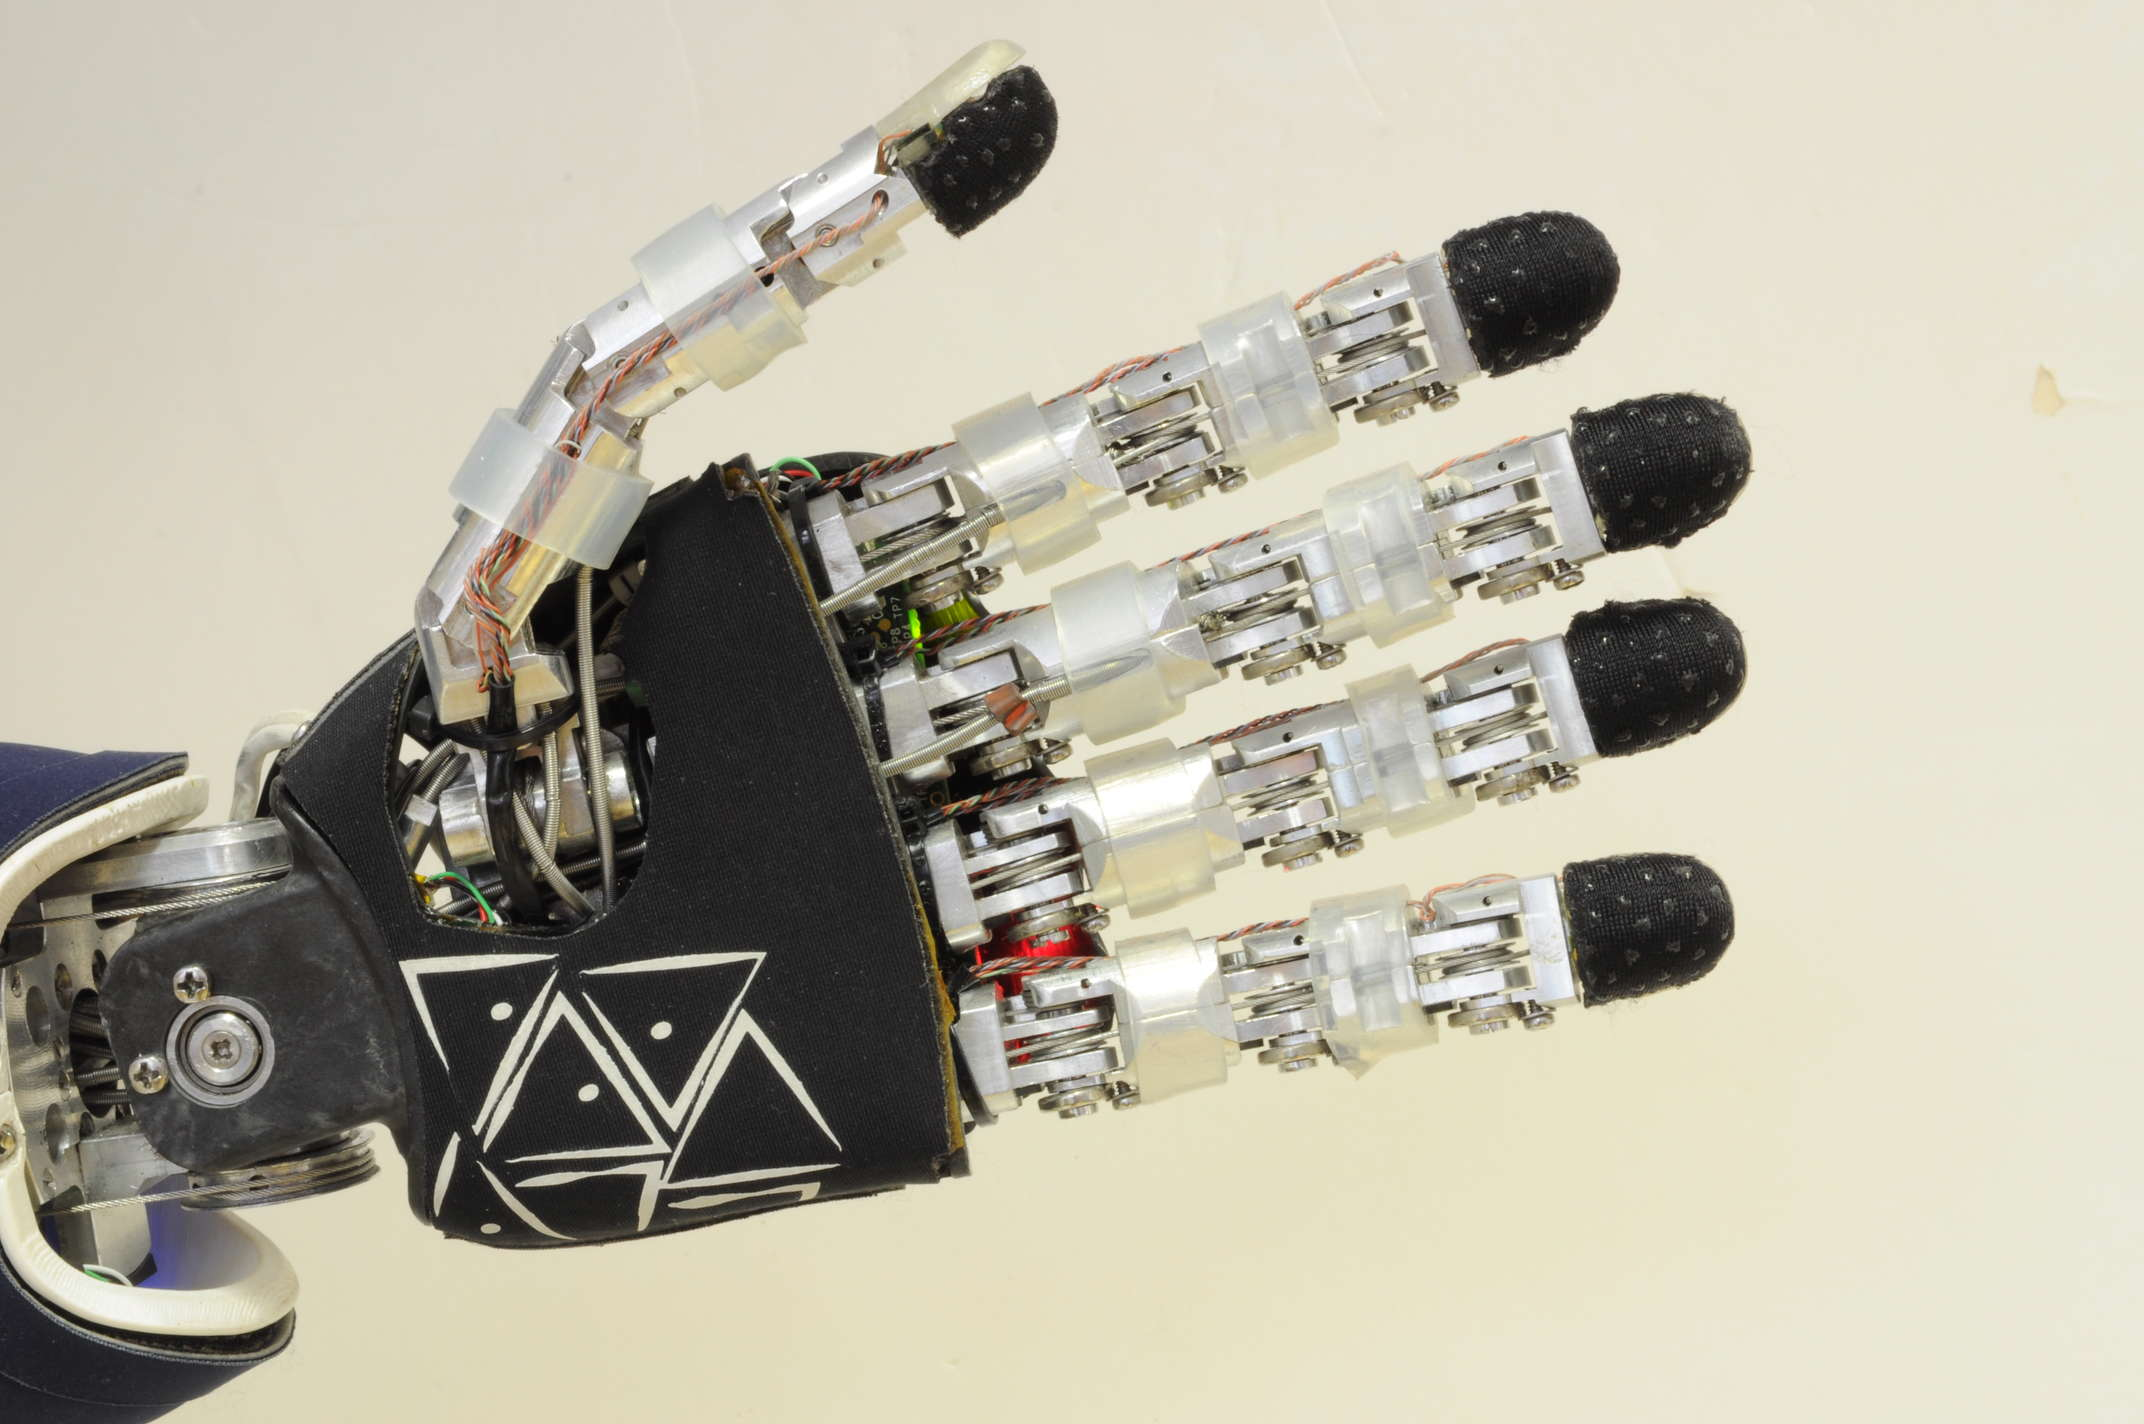
\includegraphics[width=0.3\textwidth]{persp2_straight}  } \quad
    %
    \subfloat
    {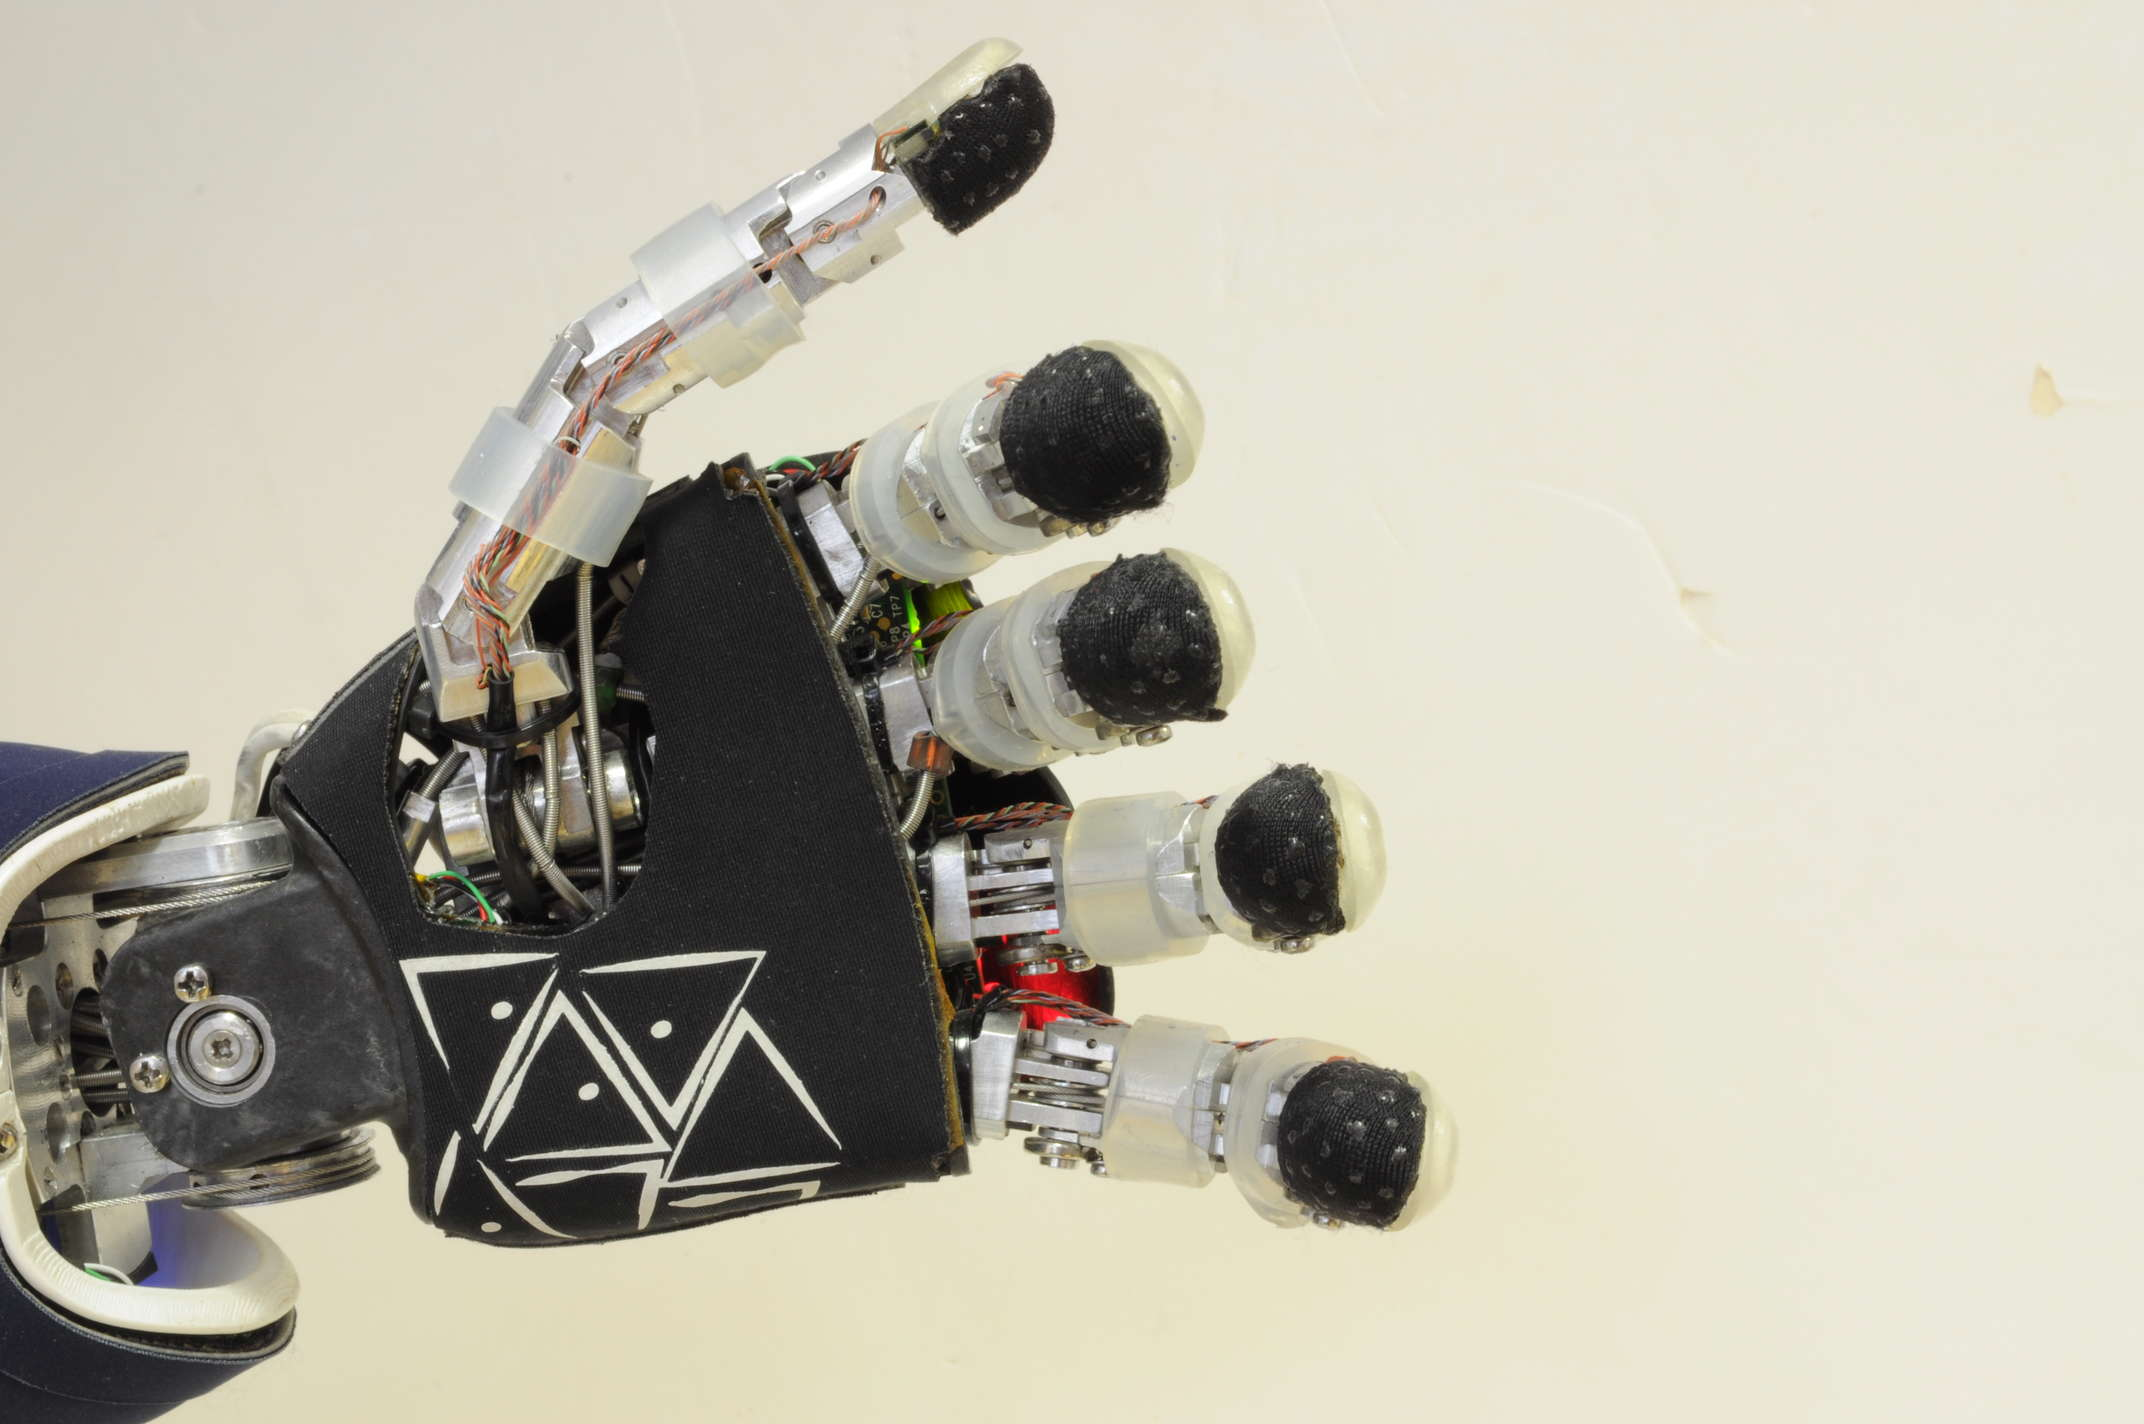
\includegraphics[width=0.3\textwidth]{persp2_bent} } \quad
    %
    \subfloat
    {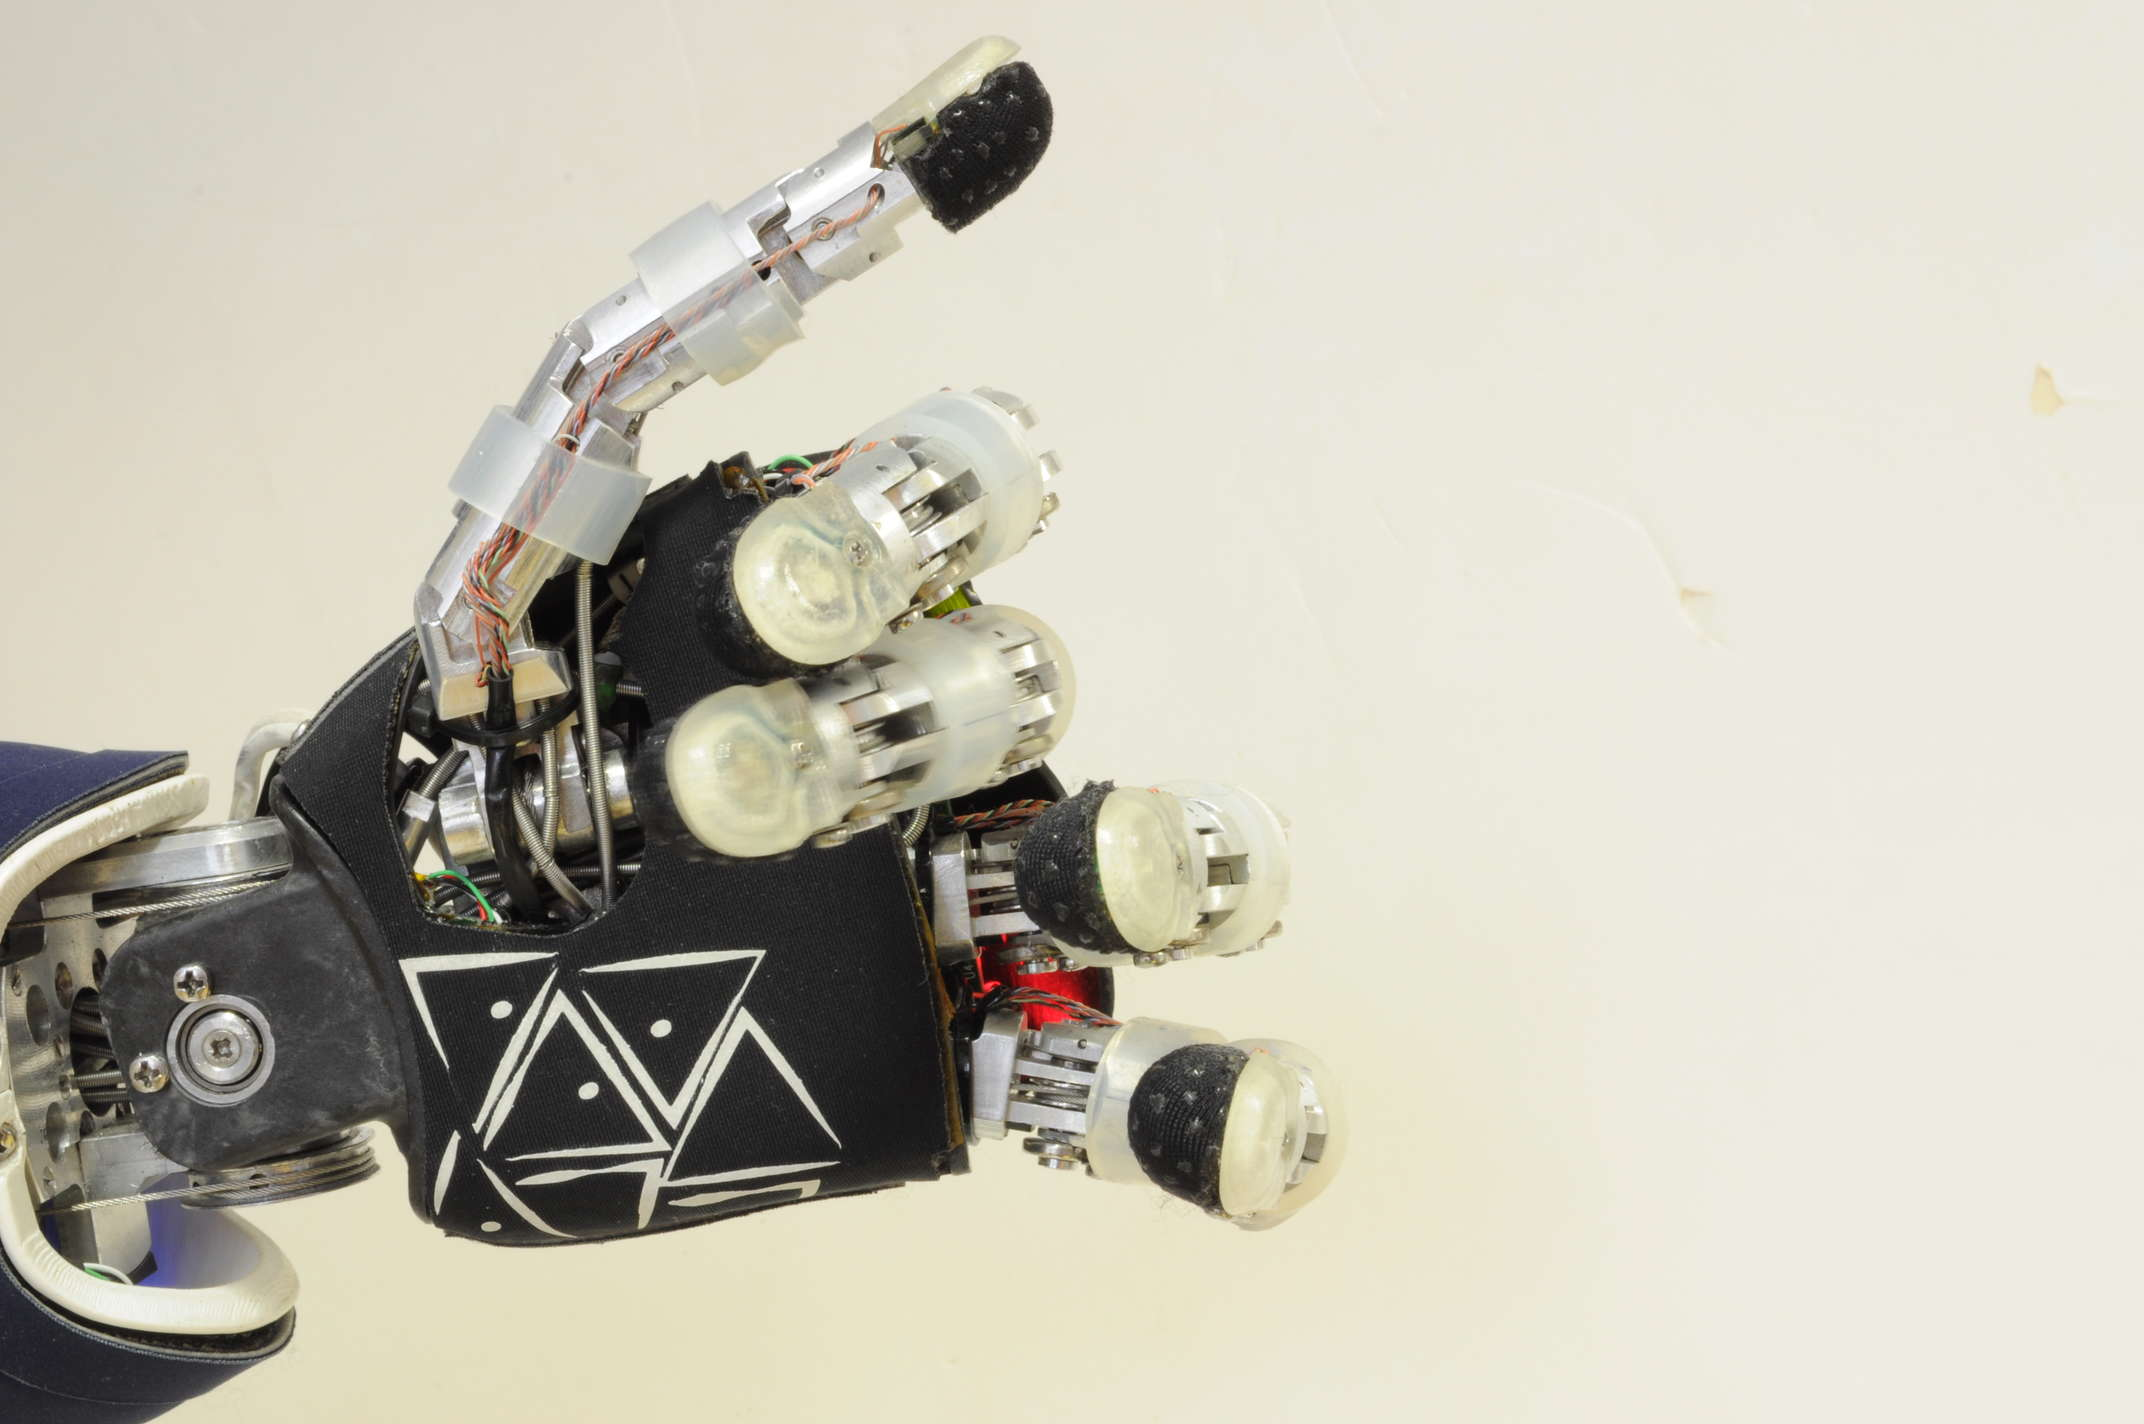
\includegraphics[width=0.3\textwidth]{persp2_fortyfive} } \\
    %
    \subfloat
    {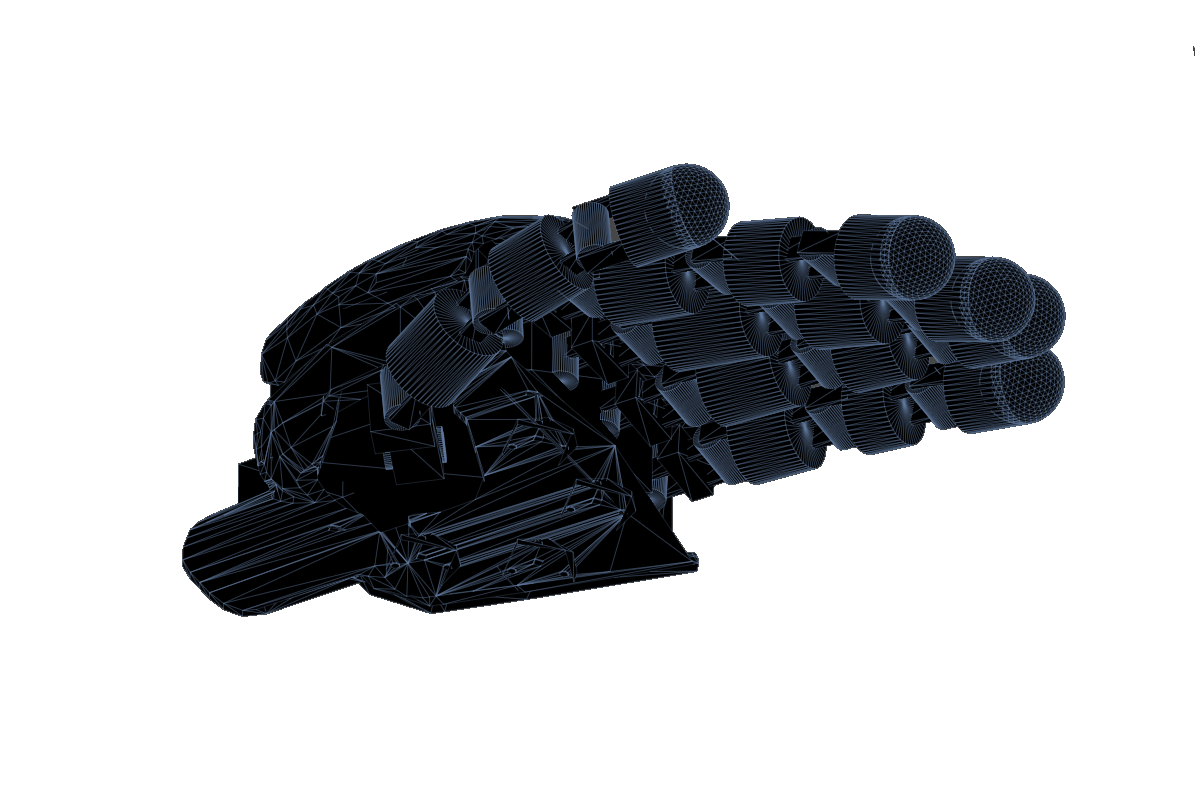
\includegraphics[width=0.3\textwidth]{handUnity_straight_persp1} } \quad
    %
    \subfloat
    {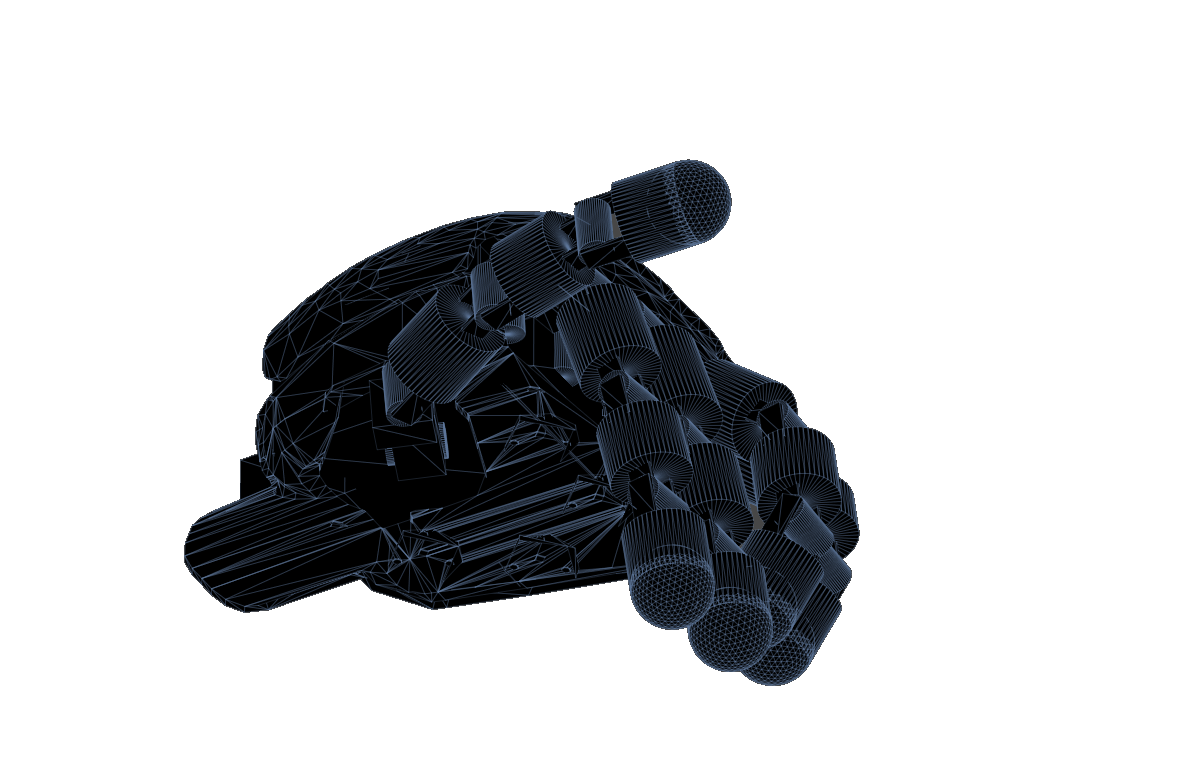
\includegraphics[width=0.3\textwidth]{handUnity_bent_persp1} } \quad
    %
    \subfloat
    {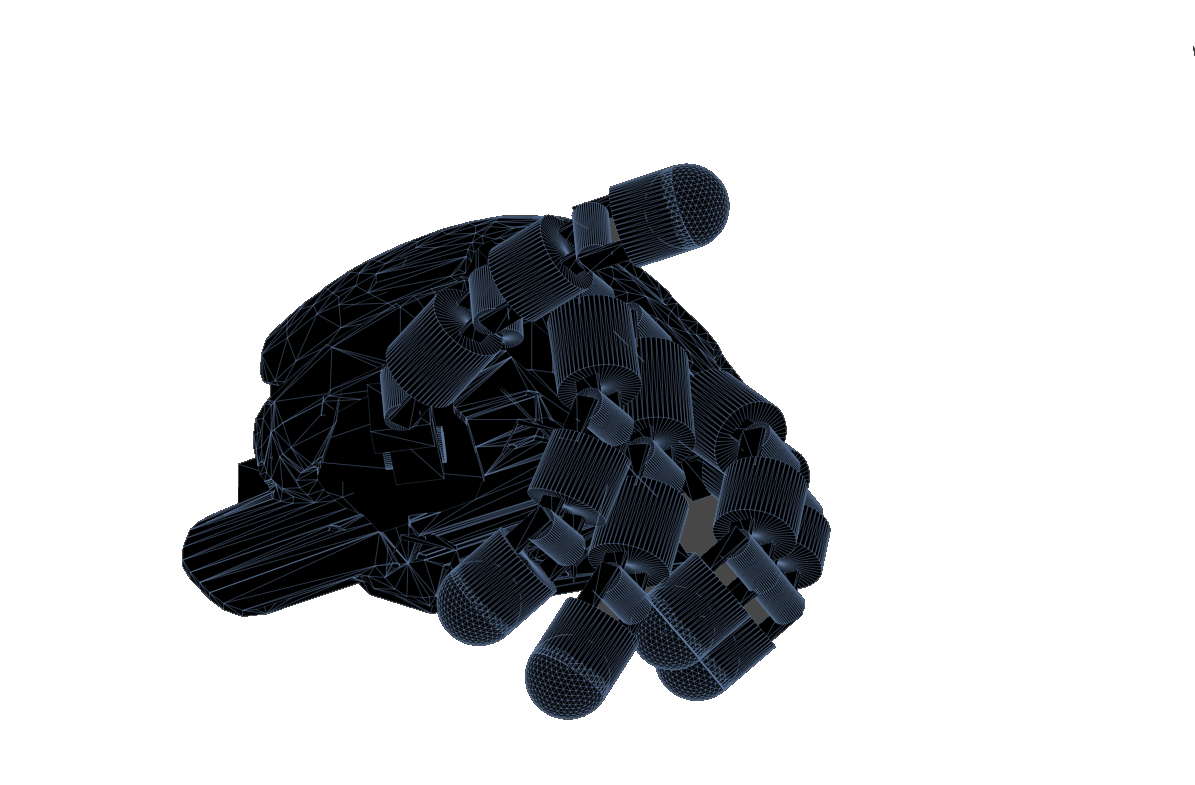
\includegraphics[width=0.3\textwidth]{handUnity_fortyFive_persp1}}
    \caption[The three robot hand postures adopted to study the hand to tool transition.]{The three robot hand postures adopted to study the hand to tool transition. Left column: straight hand; center column: bent hand; right column: arched hand. The first two rows are real robot postures seen from different viewpoints; the last row shows the simulated body schema CAD model of the top viewpoint. From the latter simulated view, we obtain the segmented silhouette contour of the hand and its shape features.}
    \label{fig:robot_hand_postures}
\end{figure*}

In particular, we adapt the model described earlier in this chapter to relate the
(i)~visual features of the agent's \emph{own hands} (i.e., in this case the manipulator node of Fig.~\ref{fig:tool:tools_computational_model} refers to the hand, not to the held object),
(ii)~visual features of an acted object located on a surface,
(iii)~a motor action, and
(iv)~the resulting effects of the action onto the object, in the sense of the physical displacement compared to the initial position.
We use three different robot hand postures, shown in Fig.~\ref{fig:robot_hand_postures}.

The setup is similar to the one described in Sec.~\ref{sec:tool:approach:model}, with the following differences:
\begin{itemize}
  \item motor control: the four directional actions performed with the robot's bare hands are: tapping an object from the left side~(with the palm of the hand), tapping an object from the right side~(with the back of the hand), pushing an object away from the agent, and pulling the object towards the agent;

  \item robot actions: the location of the acted object (i.e., the location where the robot performs an action) can be anywhere on the table, provided that it is within the reachable space of the robot end-effector, and that it satisfies geometric safety limits to avoid self-collisions. We determine this location with the visual segmentation routines described in Sec.~\ref{sec:platform:software_architecture:visual_pipeline};

  \item visual features: we incorporate a richer set of~13 features instead of~5 as was the case in Sec.~\ref{sec:tool:approach:model}.
  In addition to convexity, eccentricity, compactness, circularity, and squareness, we also compute features useful to characterize hand shapes: number of convexity defects~(i.e., number of cavities along the contour, for example the ``holes'' between fingers in a hand image), and seven central normalized moments.
  See also Sec.~\ref{tab:descriptors}.
  The raw visual features of manipulators and objects are real-valued and normalized between~0 and~1.
\end{itemize}

In our endeavor, we wish to compute the visual shape features of the robot's bare hands (for relating them with the other variables in the model), in the various hand postures, but this poses a technical challenge.
The image of a robot hand is difficult to segment from the background, and additionaly its contour is not easy to extract, given the different colors of the metal and plastic parts~(see for example the top-left hand image in Fig.~\ref{fig:robot_hand_postures}).
We bypass this problem by resorting to an internal model of the robot's hand, based on the ideas of \emph{body awareness}.

From a developmental psychology perspective, body awareness appears to be an incremental learning process that starts in early infancy~\cite{vonhofsten:2004:tcs} or probably even prenatally~\cite{joseph:2000:drev}.
Such awareness is supported by a neural representation of the body that is constantly updated with multimodal sensorimotor information acquired during motor experience and that can be used to infer the limbs' position in space and guide motor behaviors: a \emph{body schema}~\cite{berlucchi:1997:tneu}.

We use an internal model simulator from~\cite{vicente:2016:jint}.
From a technical perspective, using the simulated robot rather than the real one to obtain the hand posture visual shape, serves to filter out noise from the image processing pipeline.
Although it is not always true that we can generalize from simulation to the real robots, in this case, we adopt a graphically and geometrically precise appearance model of the robotic hand~(based on the CAD model),
therefore we can use the internal model simulation without losing generality or compromising the overall idea, as shown when visually comparing the real and simulated hands of Fig.~\ref{fig:robot_hand_postures}.

In terms of hand affordance \emph{learning}, the structure of the \ac{BN} is the \ac{PCA} one as described in the previous sections, this time putting in relationships robot manipulator (which can be the hand or the tool), acted object, motor action, and resulting effects.
Fig.~\ref{fig:tool:nets:pca2017general} shows the structure of the \ac{BN} that we train with robot self-exploration hand affordance data, using the hand postures of Fig.~\ref{fig:robot_hand_postures}.
This structure is similar to the one that gave us the best effect prediction performance in Sec.~\ref{sec:tool:approach:learning}.
In Table~\ref{tab:tool:hand_to_tool_pca_hyperparams} we list the hyper-parameters used at training time.
Thanks to the dimensionality reduction of this type of network, the number of edges and the computational complexity are also reduced.
Most importantly, this type of network reduces the amount of training data required to observe the emergence of some learning effect.

\begin{figure} % contains a figure and a table on the same page, https://tex.stackexchange.com/a/111121
\centering
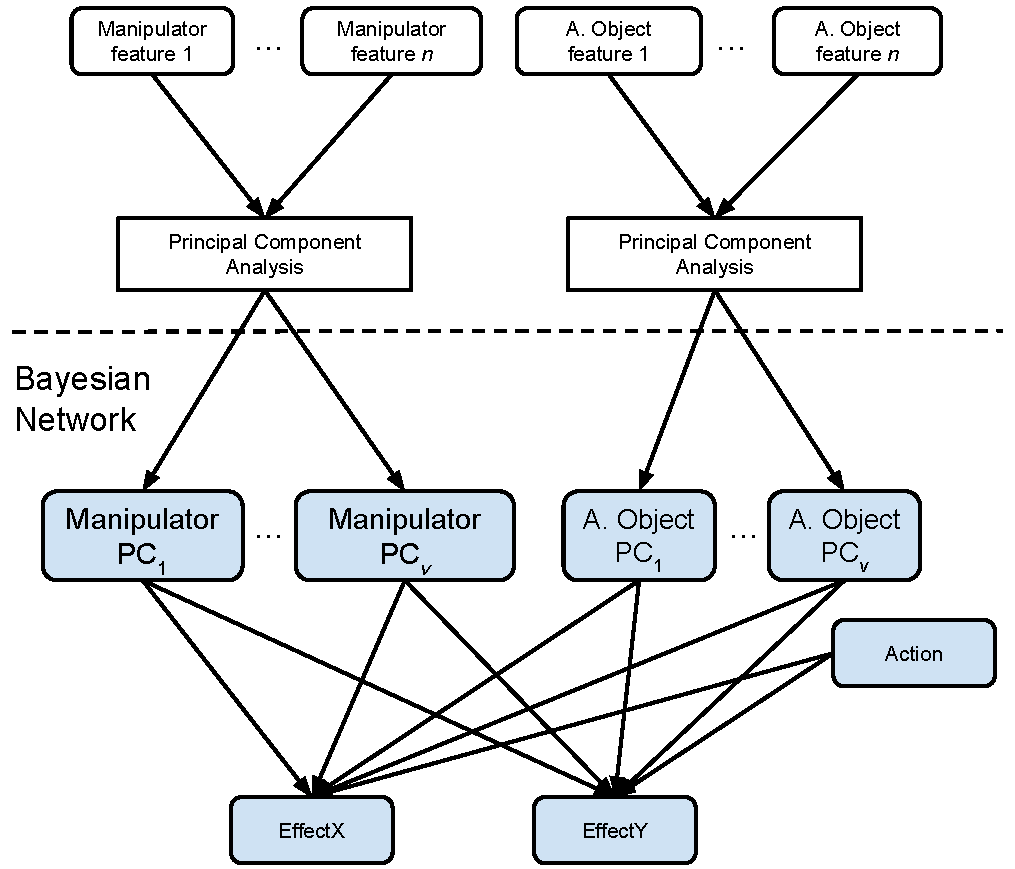
\includegraphics[width=0.9\textwidth]{pca_bn_general_icdl2017}
\caption[Dimensionality-reduced \acl{BN} structure to encode hand to tool affordances, from \cite{saponaro:2017:icdl}.]{Dimensionality-reduced \acl{BN} structure to encode hand to tool affordances, from \cite{saponaro:2017:icdl}.
A.~Object means Acted Object, Manipulator refers to the bare robot hand or to a held object (tool).
This structure was specified manually, after having empirically tried different \ac{PCA} hyper-parameters, see Table~\ref{tab:tool:hand_to_tool_pca_hyperparams}.
The \ac{PCA} dimensionality reduction is computed on the continuous vectors of the visual features.

In this case, there are two \ac{PCA} blocks: one for the manipulator visual features, one for the acted object visual features.
This is because in this work the concept of toolness was a starting hypothesis, and the focus was on the developmental transition from hand to tool affordances.}
\label{fig:tool:nets:pca2017general}
%
\captionof{table}[Hand to tool transition: hyper-parameters used to train the \acl{BN} of Fig.~\ref{fig:tool:nets:pca2017general}.]{%
Hand to tool transition: hyper-parameters used to train the \acl{BN} of Fig.~\ref{fig:tool:nets:pca2017general} for predicting the distribution of the effects.
} % end captionof
    \scriptsize
    \begin{tabular}{*{2}{l}} % left-aligned columns
    \toprule
    parameter & value (and comment) \\
    \midrule
    number of \acs{PCA} blocks                   & $2$ (one for manipulator, one for object) \\
    number of components of each \acs{PCA} block & $2$ \\
    number of discretization values (bins)       & $2$ \\
    of each \acs{PCA} component                  & \\
                                                 & \\
    number of discretization values (bins)       & $5$ \\
    of each $\Effect$ node                       & \\
                                                 & \\
    intervals (in meters) of the $\Effect$ bins  & $\interval[open left]{-\infty}{-0.06}$, $\interval[open left]{-0.06}{-0.025}$, \\
                                                 & $\interval[open left]{-0.025}{0.025}$, $\interval[open left]{0.025}{0.06}$, $\interval[open]{0.06}{\infty}$ \\
    \bottomrule
    \end{tabular}
    \label{tab:tool:hand_to_tool_pca_hyperparams}
\end{figure}

The nodes of the network are the same ones of Sec.~\ref{sec:tool:approach:learning},
but the \ac{PCA} block is different due to the following reason.

There are now two \ac{PCA} blocks: one for the manipulator visual features, one for the affected object visual features.
This is because in this work (\cite{saponaro:2017:icdl}) the concept of toolness is a starting hypothesis, and the focus is on the developmental transition from hand to tool affordances.
By contrast, in Sec.~\ref{sec:tool:approach:learning} (\cite{goncalves:2014:icdl}) there was one \ac{PCA} block for the whole original visual feature space with~12 dimensions (6 features for the manipulator or held object, and~6 for the acted object, considered jointly).
That was because the concept of toolness was not specified in that work, but was emerging from experiments.

%%%%%%%%%%%%%%%%%%%%%%%%%%%%%%%%%%%%%%%%%%%%%%%%%%%%%%%%%%%%%%%%%%%%%%%%%%%%%%%%
\section{Experimental Results}
\label{sec:tool:results}

We now show the results obtained with our tool use affordance reasoning model.
In Sec.~\ref{sec:tool:results:bns} we evaluate the various \intobj{} \ac{BN} structures both in simulation and on the real robot, then
Sec.~\ref{sec:tool:results:hand_to_tool} focuses on the experiments about hand affordances, and on the developmental link from hand affordances to tool affordances.

%%%%%%%%%%%%%%%%%%%%%%%%%%%%%%%%%%%%%%%%%%%%%%%%%%%%%%%%%%%%%%%%%%%%%%%%%%%%%%%%
\subsection{Evaluation of the \IntObj{} \aclp{BN}}
\label{sec:tool:results:bns}

To compare the multitude of possible values for the nodes of the \acp{BN} described in Sec.~\ref{sec:tool:approach:learning}, it is not feasible to collect robotic data with the real robot (for thousands of experiments), therefore we collect most data in simulation.
In particular, we gather \num{2353}~experimental trials in the iCub simulator~\cite{tikhanoff:2008:icubsim}, and 21~trials in the real iCub robot.

\begin{figure}
\newcommand{\myheight}{2.5cm}
\centering
\subfloat
{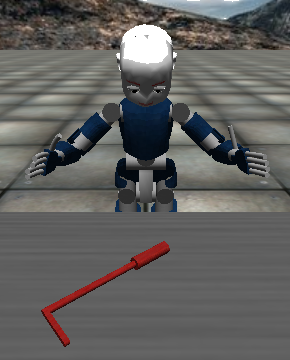
\includegraphics[height=\myheight]{tool_sim_exploration1.png} \label{fig:tool:sim_exploration:1} } \quad
%
\subfloat
{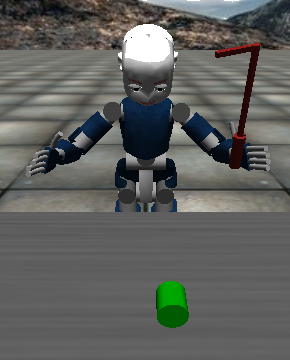
\includegraphics[height=\myheight]{tool_sim_exploration2.png} \label{fig:tool:sim_exploration:2} } \quad
%
\subfloat
{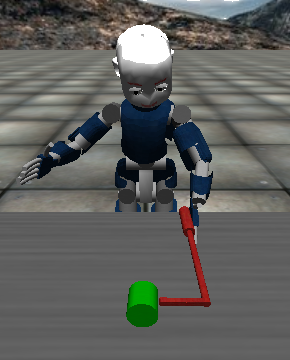
\includegraphics[height=\myheight]{tool_sim_exploration3.png} \label{fig:tool:sim_exploration:3} } \quad
%
\subfloat
{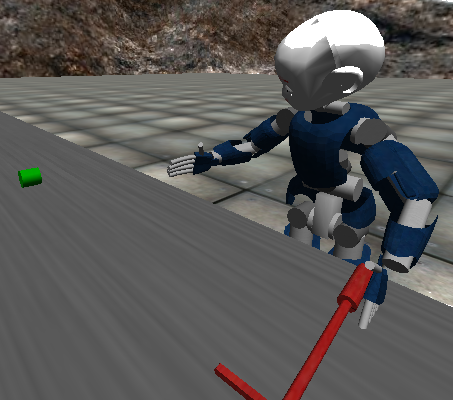
\includegraphics[height=\myheight]{tool_sim_exploration4.png} \label{fig:tool:sim_exploration:4} } \quad
%
\caption[Exploration sequence of tool use in the iCub simulator.]{Exploration sequence of tool use in the iCub simulator: (1)~the robot acquires the visual descriptors of a manipulator (held object) and its two halves while it is on the table; (2)~the robot acquires the visual descriptors of an acted object in its initial state~(position); (3)~the robot exerts one of the motor actions onto the acted object using the held manipulator; (4)~the robot observes the final position of the acted object after a fixed number of frames, permitting to compute the resulting effect compared to the initial state.}
\label{fig:tool:sim_exploration}
\end{figure}

For each trial, the \emph{experimental protocol} consists of performing one of the~4 directional movements (see Sec.~\ref{sec:tool:approach:model}) upon the acted object while holding a manipulator object (i.e., held object or tool) in the robot's hand, as shown in Fig.~\ref{fig:tool:sim_exploration}.
Both objects are chosen from a set of~8 possibilities displayed in Fig.~\ref{fig:tool:sim_objects}).

Of the whole set of experiments, a part is used to learn the proposed \acl{BN} models and a part is used for testing, as described in Sec.~\ref{sec:tool:approach:learning}.

\begin{figure}
\centering
\subfloat[][Ball.]
{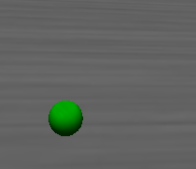
\includegraphics[width=0.2\textwidth]{tool_sim_objects_1-ball.png} \label{fig:tool:sim_objects:ball} } \quad
%
\subfloat[][Cube.]
{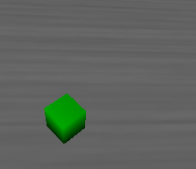
\includegraphics[width=0.2\textwidth]{tool_sim_objects_2-cube.png} \label{fig:tool:sim_objects:cube} } \quad
%
\subfloat[][Cylinder.]
{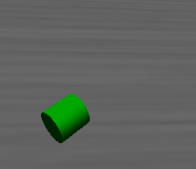
\includegraphics[width=0.2\textwidth]{tool_sim_objects_3-cylinder.png} \label{fig:tool:sim_objects:cylinder} } \quad
%
\subfloat[][Stick.]
{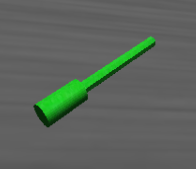
\includegraphics[width=0.2\textwidth]{tool_sim_objects_4-stick.png} \label{fig:tool:sim_objects:stick} } \\
%
\subfloat[][L-stick.]
{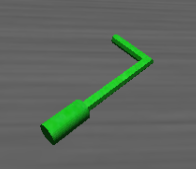
\includegraphics[width=0.2\textwidth]{tool_sim_objects_5-L-stick.png} \label{fig:tool:sim_objects:L-stick} } \quad
%
\subfloat[][Bone.]
{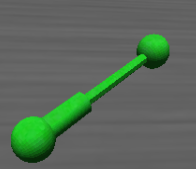
\includegraphics[width=0.2\textwidth]{tool_sim_objects_6-bone.png} \label{fig:tool:sim_objects:bone} } \quad
%
\subfloat[][Umbrella.]
{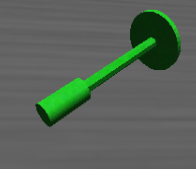
\includegraphics[width=0.2\textwidth]{tool_sim_objects_7-umbrella.png} \label{fig:tool:sim_objects:umbrella} } \quad
%
\subfloat[][Fork.]
{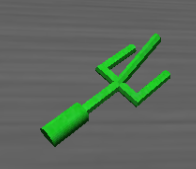
\includegraphics[width=0.2\textwidth]{tool_sim_objects_8-fork.png} \label{fig:tool:sim_objects:fork} }
%
\caption[Objects used in robot simulation to train affordance \aclp{BN}.]{Objects used in robot simulation to train affordance \aclp{BN}. Object~\subref{fig:tool:sim_objects:fork} is only used
in one of the evaluation tests of Sec.~\ref{sec:tool:results:bns:effect_prediction}.%
}
\label{fig:tool:sim_objects}
\end{figure}

For our tests, we use two \emph{evaluation criteria}:

\begin{description}
\item[Accuracy:] defined as the number of correct predictions (e.g., discrete predictions of effect, or tool, or action, depending on the query) over the number of total predictions.

\item[Distance:] defined as the absolute difference
between the prediction (e.g., discrete predictions of effect, or tool, or action, depending on the query) and the real value (i.e., \acl{GT}, also discrete).
In Tables~\ref{tab:tool:scores:splitting} and~\ref{tab:tool:scores:leave_one_out}
it is shown as a percentage, relative to the maximum possible distance.
\end{description}

%%%%%%%%%%%%%%%%%%%%%%%%%%%%%%%%%%%%%%%%%%%%%%%%%%%%%%%%%%%%%%%%%%%%%%%%%%%%%%%%
\subsubsection{Effect Prediction}
\label{sec:tool:results:bns:effect_prediction}

We evaluate the \acp{BN} regarding their capability of predicting effects, given two objects' visual descriptors and the action performed with them, with previously unseen test data.
To do this we use two different evaluation techniques: (i)~data splitting and (ii)~leave-one-out validation.

The first evaluation consists of randomly \emph{splitting} the data in a training set with $80\%$~of observations, the remaining~$20\%$ for testing.
The exploration data is relative to the~\num{1663} trials corresponding to the seven objects of Fig.~\ref{fig:tool:sim_objects:ball}--\ref{fig:tool:sim_objects:umbrella}.
Results are presented in Table~\ref{tab:tool:scores:splitting}.
The original baseline network is the one with the lowest performance: due to its huge complexity, this network does not generalize well what it learned.
13.55\%~of the time, this network made a random prediction because an event where all the instantiated variables were seen with the exact same values observed in the test data was never seen during training.
The \ac{PCA} network yields a good score, because it has the smallest complexity of all the networks considered.
However, the two networks obtained with \StructureLearning{} (i.e., BDe and K2) provide very similar results, being the networks with the best performance on the test data.

\begin{table}
\caption[Data splitting scores when randomly selecting 80\% of observations as training data, the remaining observations as test data.]{Data splitting scores when randomly selecting 80\% of observations as training data, the remaining observations as test data.
Accuracy: higher is better.
Distance: lower is better.
R.p. stands for random predictions.}
\label{tab:tool:scores:splitting}
\centering
\begin{tabular}{p{0.21\columnwidth}    *{4}{p{0.13\columnwidth}}} % five columns
\toprule
        & Baseline (13.55\% r.p.) & \ac{PCA} (0\%~r.p.) & \StructureLearning{} BDe (0\%~r.p.) & \StructureLearning{} K2 (0\%~r.p.) \\
\midrule
Accuracy            & $75.90\%$   & $80.57\%$   & $83.28\%$ & $\textbf{83.73\%}$ \\
Distance            &  $9.11\%$   &  $6.10\%$   &  $\textbf{5.12\%}$ &  $\textbf{5.12\%}$ \\
\bottomrule
\end{tabular}
\end{table}

The second evaluation is a \emph{leave-one-out} validation, using the same networks as in the data splitting one, but the unseen object of Fig.~\ref{fig:tool:sim_objects}~\subref{fig:tool:sim_objects:fork} as test data (690~samples).
Results are shown in Table~\ref{tab:tool:scores:leave_one_out}.
The \ac{PCA} network has the best performance: being the least complex network makes it the most capable network for generalization to unseen objects.
The performance of the other networks gets significantly worse, showing that these networks are too dependent on the training data (overfitting), so their use on the real robot with a changing environment should be accompanied with an online \StructureLearning{} and parameter learning algorithm, which we do not do (the K2 and BDe structures are learned offline).

\begin{table}
\caption[Leave-one-out scores, testing networks against an object unseen during training.]{Leave-one-out scores, testing networks against an object unseen during training.
Accuracy: higher is better.
Distance: lower is better.
R.p. stands for random predictions.}
\label{tab:tool:scores:leave_one_out}
\centering
\begin{tabular}{p{0.21\columnwidth}    *{4}{p{0.13\columnwidth}}} % five columns
\toprule
        & Baseline (57.25\% r.p.) & \ac{PCA} (0\% r.p.) & \StructureLearning{} BDe (52.61\% r.p.) & \StructureLearning{} K2 (53.04\% r.p.) \\
\midrule
Accuracy           & $44.20\%$   & $\textbf{73.91\%}$   & $48.42\%$ & $47.93\%$ \\
Distance           & $25.60\%$   &  $\textbf{7.28\%}$   & $23.72\%$ & $23.97\%$ \\
\bottomrule
\end{tabular}
\end{table}

%%%%%%%%%%%%%%%%%%%%%%%%%%%%%%%%%%%%%%%%%%%%%%%%%%%%%%%%%%%%%%%%%%%%%%%%%%%%%%%%
\subsubsection{Generalization from Simulation to Reality}
\label{sec:tool:results:bns:sim_to_real}

In this experiment, the robot executes the left lateral tap action while holding a straight stick.
It repeats this action~10 times acting on a ball,~11 times acting on a box.
From each iteration, we acquire the \acf{GT}.
The \ac{GT} is the discrete index of the displacement bin where the object finished after being acted upon and moving: see p.~\pageref{para:effects} for the names of the bins, Table~\ref{tab:tool:tool_pca_hyperparams} for the parameters.
Then, we compare the \ac{GT} to the computed prediction of the resulting effect, given the manipulator and acted objects, by the K2 and \ac{PCA} network.

In this experiment, we do not present results of the baseline and the BDe networks: they provide random answers, i.e., equal probability for all values, because those networks' structures do not represent well the exact combination of observations in the experiment.

Results for the query $p(\Effect | \parents(\Effect))$, where $\Effect$ is~$\EffectX$ or~$\EffectY$, and the \acp{GT}, are shown together in Table~\ref{tab:tool:prediction:all}.

% custom column type to Hide a column
% https://tex.stackexchange.com/a/26482
% https://tex.stackexchange.com/a/16607
\newcolumntype{H}{>{\setbox0=\hbox\bgroup}c<{\egroup}@{}}

\begin{table}
\raggedleft
\caption[Comparison between \acf{GT} and effect prediction by K2 and \acs{PCA} networks.]{Comparison between \acf{GT} and effect prediction by K2 and \acs{PCA} networks.
See p.~\pageref{para:effects} for the abbreviations of the five effect bins, Table~\ref{tab:tool:tool_pca_hyperparams} for the parameters.
\acs{PCA} provides better matches for the ball experiments, K2 for the box ones.
Overall, \acs{PCA} has a match distance $7.3\%$ higher than K2. }
\label{tab:tool:prediction:all}
\tiny
\begin{tabularx}{\textwidth}{ l *{6}{X} *{15}{H} } % left-aligned, 6 'X' (auto-spaced, see tabularx manual), 15 Hidden
\toprule
 & \multicolumn{3}{c}{VN} & \multicolumn{3}{c}{LN} \\
\cmidrule(lr){2-4} \cmidrule(lr){5-7}
 & \ac{GT} & K2 & \ac{PCA} & \ac{GT} & K2 & \ac{PCA} & \ac{GT} & K2 & \ac{PCA} & \ac{GT} & K2 & \ac{PCA} & \ac{GT} & K2 & \ac{PCA} & K2 &
  \\ % some columns are hidden by the custom H column type
\midrule
\toolPredictionBigTabularData
\bottomrule
\end{tabularx}

\bigskip
%
\begin{tabularx}{\textwidth}{ H *{6}{H} *{11}{X} }
\toprule
& & & & &  &  & \multicolumn{3}{c}{NM} & \multicolumn{3}{c}{LP} & \multicolumn{3}{c}{VP} & \multicolumn{2}{c}{match distance} \\ % hide first columns manually, add some empty columns to shift the bin names to the right (hack)
        \cmidrule(lr){1-10} \cmidrule(lr){11-13} \cmidrule(lr){14-16} \cmidrule(lr){17-18} % hide first columns manually; 1-10 instead of 8-10 (hack)
 & \ac{GT} & K2 & \ac{PCA} & \ac{GT} & K2 & \ac{PCA} & \ac{GT} & K2 & \ac{PCA} & \ac{GT} & K2 & \ac{PCA} & \ac{GT} & K2 & \ac{PCA} & K2 &
\ac{PCA}  \\
\midrule
\toolPredictionBigTabularData
\bottomrule
\end{tabularx}
\end{table}

We evaluate how well the predictions match the \acp{GT} by computing the \emph{match distance}~\cite{rubner:2000:earth} between their histogram distributions.
Being a cross-bin dissimilarity measure, the match distance is suited to cases where the bin order matters.
Our bin order for the effects (VN,LN,NM,LP,VP), as defined on p.~\pageref{para:effects}, places more similar displacements in neighbor bins.
The maximum value of the distance, in our case, is $d_{\text{MAX}}=4$, the distance between histograms $(1,0,0,0,0)$ and $(0,0,0,0,1)$.
It is a special case of the Earth Mover's Distance~\cite{rubner:2000:earth}, so it can be interpreted as the amount of mass transported between bins times their distance, to transform one histogram into the other.

Both the \ac{PCA} network and the K2 structure provide acceptable results (average match distances below~$10\%$ of~$d_{\text{MAX}}$), with K2 being slightly more accurate (about~$7\%$ lower match distances), although the K2 structure has the peculiarity of the $\EffectX$ node being conditionally independent from acted object features (see Fig.~\ref{fig:tool:nets:k2}).
This explains why the K2~$\EffectX$ rows of Table~\ref{tab:tool:prediction:all} have equal values, regardless of the acted object.

%%%%%%%%%%%%%%%%%%%%%%%%%%%%%%%%%%%%%%%%%%%%%%%%%%%%%%%%%%%%%%%%%%%%%%%%%%%%%%%%
\subsubsection{Tool Selection}
\label{sec:tool:results:bns:tool_selection}

\begin{figure}
\centering
\subfloat[]
{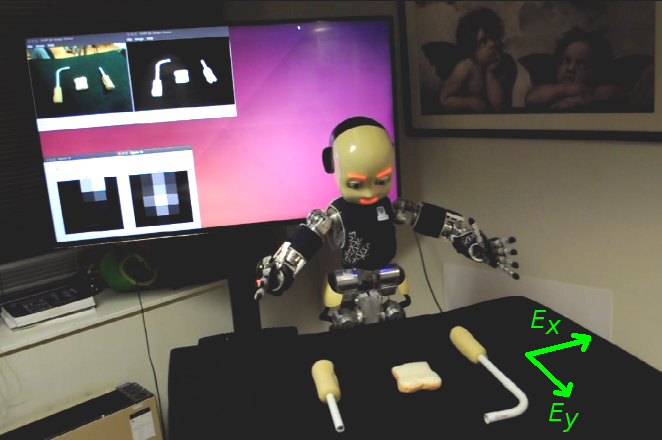
\includegraphics[width=0.24\linewidth, clip, trim=8.5cm 0cm 2cm 0cm]{iCub_selecting_between_two_tools2} \label{fig:iCub_selecting_between_two_tools:photo} } \quad
%
\subfloat[]
{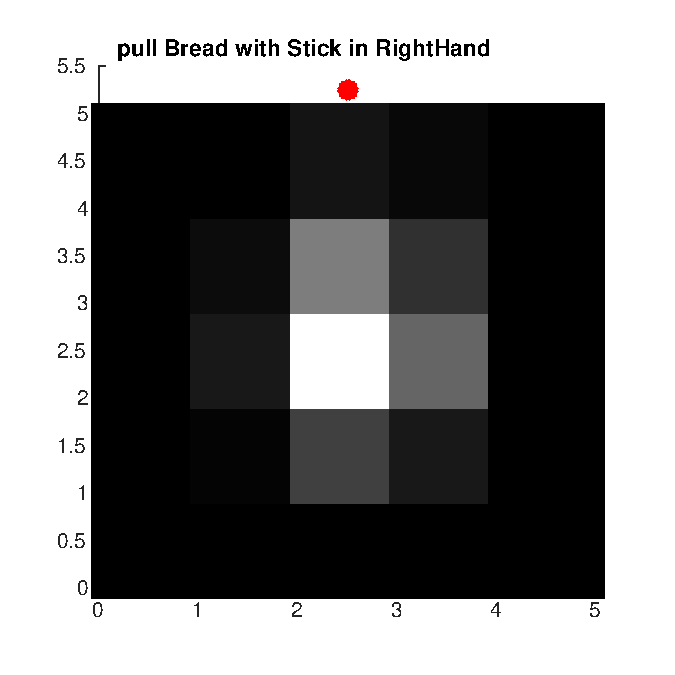
\includegraphics[width=0.26\linewidth]{pull_with_Stick} \label{fig:iCub_selecting_between_two_tools:pStick} } \quad
%
\subfloat[]
{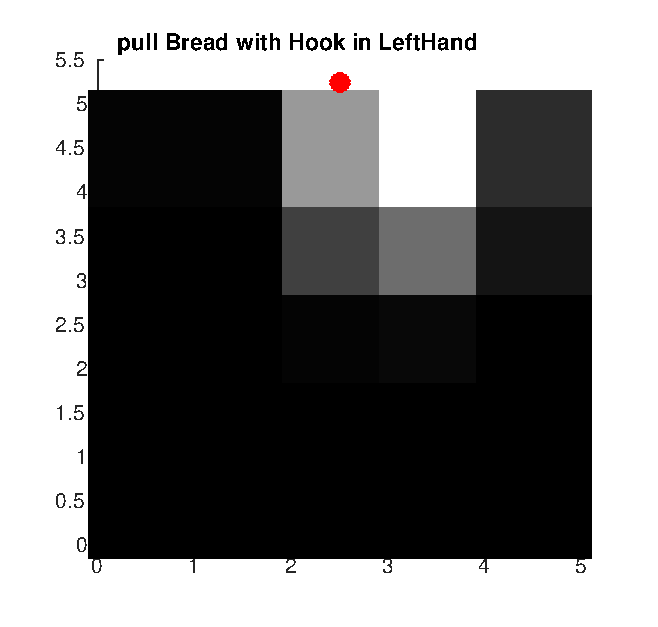
\includegraphics[width=0.26\linewidth]{pull_with_Hook} \label{fig:iCub_selecting_between_two_tools:pHook} } \quad
%
\subfloat
{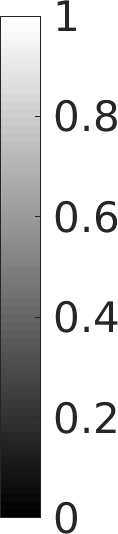
\includegraphics[width=0.05\linewidth]{colorbar_gray-trimmed} }
\caption[The iCub robot using affordance reasoning to select the most appropriate tool for achieving a given action.]{(a):~the iCub robot using affordance reasoning to select the most appropriate tool for achieving a given action, i.e., pulling the bread closer to the agent.
(b--c):~effect prediction probabilities of the bread motion using the tools, where the robot location is marked with a red dot, and the table area is divided into a grid of squares.}
\label{fig:iCub_selecting_between_two_tools}
\end{figure}

In the example of
Fig.~\ref{fig:iCub_selecting_between_two_tools}, the robot has to \emph{select the most appropriate tool}
for pulling
the bread object
closer to it.
Figs.~\ref{fig:iCub_selecting_between_two_tools:pStick} and~\ref{fig:iCub_selecting_between_two_tools:pHook} show the motion effect predictions (posterior probabilities) using the Stick and the Hook tools, respectively.
In the figures, the table is discretized into a grid, and the robot location is represented by the red dot.
The values of the effect predictions represented by the figures are the following:
\begin{equation} \label{eq:posterior_pull_with_stick}
\begin{split}
p(\EffectX, \EffectY \given A=\text{pull}, T=\text{Stick visual features}, \\
O=\text{Bread visual features}) = \\
    \begin{bmatrix*}[l] % left-aligned columns
    0 &   0.0030 &   0.0290 &   0.0118 &        0 \\
    0 &   0.0185 &   0.1780 &   0.0722 &        0 \\
    0 &   0.0374 &   0.3602 &   0.1461 &        0 \\
    0 &   0.0099 &   0.0952 &   0.0386 &        0 \\
    0 &        0 &        0 &        0 &        0
    \end{bmatrix*},
\end{split}
\end{equation}

\begin{equation} \label{eq:posterior_pull_with_hook}
\begin{split}
p(\EffectX, \EffectY \given A=\text{pull}, T=\text{Hook visual features}, \\
O=\text{Bread visual features}) = \\
    \begin{bmatrix*}[l] % left-aligned columns
    0.0085 &   0.0085 &   0.2257 &   0.3704 &   0.0681 \\
    0.0037 &   0.0037 &   0.0973 &   0.1597 &   0.0294 \\
    0.0003 &   0.0003 &   0.0083 &   0.0136 &   0.0025 \\
    0      &   0      &   0      &   0      &   0 \\
    0      &   0      &   0      &   0      &   0
    \end{bmatrix*}.
\end{split}
\end{equation}

The posterior distributions in~\eqref{eq:posterior_pull_with_stick} and~\eqref{eq:posterior_pull_with_hook} show the expected pulling movement effects when using the Stick or the Hook, respectively.
The latter achieves higher values along the desired direction (i.e., in the values along the first two rows, corresponding to the motion of the acted object Bread towards the agent, as desired when performing a pulling action).
Therefore, the robot selects the Hook.
This happens because the Hook possesses shape characteristics similar to the ones of tools that have achieved successful \emph{pull} actions during learning, therefore it yields a higher probability of the desired motion compared to the Stick.

%%%%%%%%%%%%%%%%%%%%%%%%%%%%%%%%%%%%%%%%%%%%%%%%%%%%%%%%%%%%%%%%%%%%%%%%%%%%%%%%
\subsection{Evaluation of the Hand to Tool Transition}
\label{sec:tool:results:hand_to_tool}

We train a probabilistic model of hand affordances, relating visual features of (i)~different robotic hand postures and (ii)~different objects, with the resulting effects caused by the robot motor actions onto such objects.
Training data are collected during several experiments in which the iCub robot (see Sec.~\ref{sec:platform:icub}) performs manual actions on objects located on a table.
We publicly release a novel dataset of hand posture affordances\footnote{\url{https://github.com/vislab-tecnico-lisboa/affordance-datasets} \label{footnote:hand_aff_dataset}}, and we test it for generalization against an available dataset of tool affordances~\cite{dehban:2016:eccvws}.

We now present the results obtained from our hand affordance model, and we assess its performance.

%%%%%%%%%%%%%%%%%%%%%%%%%%%%%%%%%%%%%%%%%%%%%%%%%%%%%%%%%%%%%%%%%%%%%%%%%%%%%%%%
\subsubsection{Hand Affordances Dataset}

Our experimental data is obtained by making manipulation experiments on an iCub humanoid robot, in a setup like the one shown in Fig.~\ref{fig:iCub_with_different_hand_postures}, using its left arm for data collection.
We consider 4~motor actions A (tapFromRight, tapFromLeft, pull, push), 2~objects O (lego piece, pear), 3~hand postures H (straight fingers, bent fingers, arched fingers; shown in Fig.~\ref{fig:robot_hand_postures}).
We extract the visual features from both O and H (before performing the actions).
The dataset is publicly available: see footnote~\footref{footnote:hand_aff_dataset} on p.~\pageref{footnote:hand_aff_dataset}.

\begin{figure*}
    \subfloat[][Motion caused with the robot \emph{hands} when using different actions and hand postures, as observed when interacting with 2~objects multiple times in our experiments.]
    { 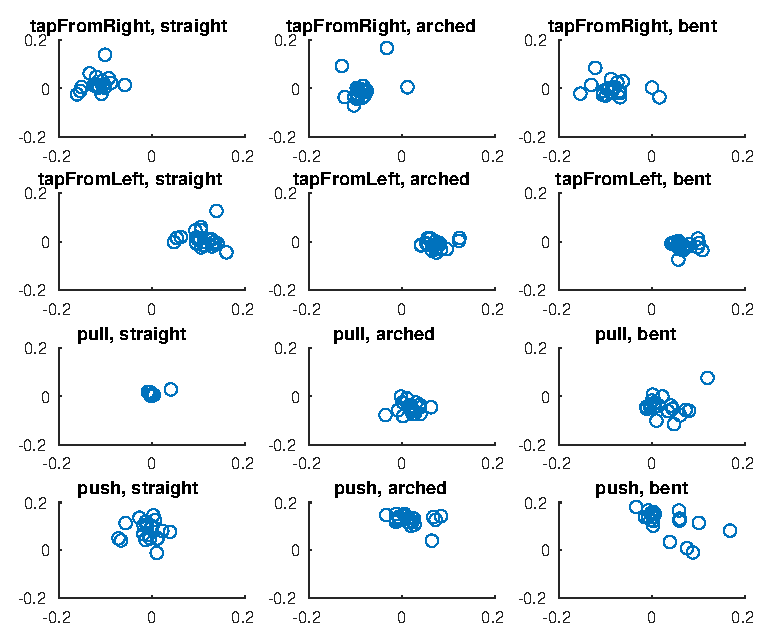
\includegraphics[width=0.8\textwidth]{all_hand_effects_2obj} \label{fig:hand_to_tool_effect_data:hands} } \\
    %
    \subfloat[][Motion caused with \emph{tools} when using different actions and tool types, taken from~\cite{dehban:2016:eccvws}. Here we show only the interactions with 2~objects, to be consistent with Fig.~\ref{fig:hand_to_tool_effect_data:hands}.]
    { 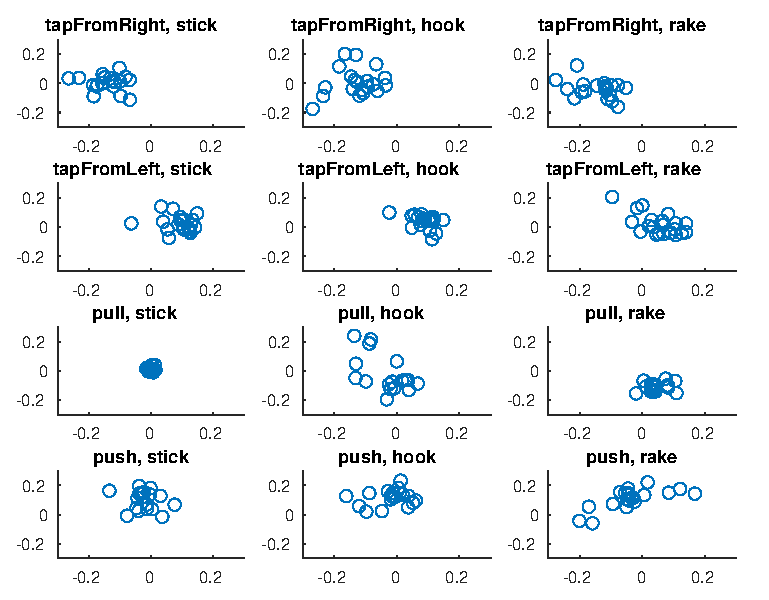
\includegraphics[width=0.8\textwidth]{all_tool_effects_2obj} \label{fig:hand_to_tool_effect_data:tools} }
    \caption[Motion caused by different robotic manipulators~(hands and tools) when using different actions and manipulator morphologies.]{Motion caused by different robotic manipulators~(hands and tools) when using different actions and manipulator morphologies: in Fig.~\ref{fig:hand_to_tool_effect_data:hands} we use different hand postures, whereas in Fig.~\ref{fig:hand_to_tool_effect_data:tools} we vary tool types for comparison. Each plot displays the geometrical displacement along horizontal and vertical direction~(in meters, measured from the object initial position) from the point of view of the robot~(the robot is at the~0 in the x-axis marker). For example, tapping an object from the right~(tapFromRight action) usually results in making the object shift to the left direction; pulling an object closer only works if the manipulator morphology is appropriate.}
    \label{fig:hand_to_tool_effect_data}
\end{figure*}

In Fig.~\ref{fig:hand_to_tool_effect_data} we show the distributions of the motion effects onto acted objects caused by the robot influence when it touches objects with its manipulator.
In particular, Fig.~\ref{fig:hand_to_tool_effect_data:hands} shows the effects of using the different hand postures.
For comparison, Fig.~\ref{fig:hand_to_tool_effect_data:tools} depicts the effect of using the elongated tools (Fig.~\ref{fig:dehban_tools}) on the same objects.
Visual inspection reveals the similarities in the effect of using tools or hands, for example, tapping from left usually results in the object moving to the right.
Another prominent similarity is that pulling with a stick or with the straight hand posture causes only minimal movement.

\begin{figure}
    \centering
    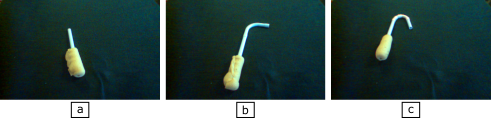
\includegraphics[width=0.9\textwidth]{atabak_tools}
    \caption[Hand to tool transition: the three baseline tools used in~\cite{dehban:2016:eccvws}.]{Hand to tool transition: the three baseline tools used in~\cite{dehban:2016:eccvws},
    (a)~stick, (b)~rake and (c)~hook. They provide different affordances when grasped by the hand of the robot and employed for performing motor actions onto objects. In this chapter, we consider these tool affordances as a comparison term to assess our novel hand affordances.}
    \label{fig:dehban_tools}
\end{figure}

We also do data augmentation on the Hand Affordances Dataset.
We assume that the affordance of an object and of a robot manipulator is viewpoint-invariant.
By exploiting this notion, it is possible to artificially augment the trials data using \emph{multiple views} of manipulators and objects.
In all of the following experiments, we have used at least 10~viewpoints of each object and manipulator, effectively multiplying the number of available samples by more than~100 times.

%%%%%%%%%%%%%%%%%%%%%%%%%%%%%%%%%%%%%%%%%%%%%%%%%%%%%%%%%%%%%%%%%%%%%%%%%%%%%%%%
\subsubsection{Effect Prediction}
\label{sec:tool:results:hand_to_tool:effect_prediction}

One way to assess the quality of the learned \ac{BN} of Fig.~\ref{fig:tool:nets:pca2014} is to predict the effect distribution, given the descriptors of manipulator, object, and action, i.e., the direct application of~\eqref{eq:effect_query}.
As before, we have empirically divided the effect distribution along each axis into five bins~(a list of the hyper-parameters that we used for training our network is reported in Table~\ref{tab:tool:hand_to_tool_pca_hyperparams} for reproducibility).
We use the accuracy metric from Sec.~\ref{sec:tool:results:bns}, which is the fraction of correct predictions by the network (i.e., when it predicts the correct effect bin out of five) among the total number of predictions performed.
Since there exist two axis directions, a random predicting machine would be correct~1/25 of the time.
At the end of this assessment, we divide by the number of total predictions performed.

\begin{table}
\caption[Hand to tool transition: accuracy of the \acl{BN} with different training and test data.]{Hand to tool transition: accuracy of the \acl{BN} with different training and test data. Chance level is 4\% (see text).}
\label{tab:tool:accuracy_hand_tool}
\centering
\begin{tabular}{*{3}{r}} % three right-aligned columns
\toprule
training set & test set   & accuracy \\
\midrule
80\% hand    & 20\% hand  & 72\% \\
80\% tool    & 20\% tool  & 58\% \\
100\% hand   & 100\% tool & 53\% \\
\bottomrule
\end{tabular}
\end{table}

Using the same network parameters but training with different data, we obtain the accuracy scores reported in Table~\ref{tab:tool:accuracy_hand_tool}.
To explain these scores, we note that motor control on the iCub is noisy, and actions on this platform are not deterministic or repeatable~(e.g., when commanding the robot twice starting from an initial position, the same motor command can produce two slightly different configurations).
Even so, in Table~\ref{tab:tool:accuracy_hand_tool} and in Fig.~\ref{fig:hand_to_tool_effect_data} we see that tool effects are more varied than hand effects, making tools less reliable~(i.e., more noisy) than hands.
Nevertheless, by only training on the hand data, we obtain an accuracy that is comparable with the case where the network is trained on tool data, demonstrating the generalization of our proposed method.

%%%%%%%%%%%%%%%%%%%%%%%%%%%%%%%%%%%%%%%%%%%%%%%%%%%%%%%%%%%%%%%%%%%%%%%%%%%%%%%%
\subsubsection{Tool Selection from Hand Affordance Knowledge}

One question that we wish to investigate is the following: if an agent gains the knowledge of how its hand postures can affect the environment, can it generalize this knowledge to other tools which look similar to its hands?
To answer this question in the scope of the presented scenario, we conduct the following experiment.
We suppose that an agent has defined a goal, for example to pull an object towards itself.
It knows that the correct action for this task will be to \emph{pull} ($A = \text{pull}$), however the object is out of the hand's reach and one of the presented tools of Fig.~\ref{fig:dehban_tools} must be selected for the task.

In this scenario, an agent looks at the available tools and at the acted object and performs a mental simulation of the known action along the two effect displacement directions:
  \begin{align*}
    p(\EffectX &\given A=\text{pull}, M=\text{tool visual features}, O=\text{object visual features}), \\
    p(\EffectY &\given A=\text{pull}, M=\text{tool visual features}, O=\text{object visual features}), \\
               &\text{for each tool available in the scene}.
  \end{align*}

The above expressions return a posterior distribution, in the form of a $5 \times 5$ matrix, because of the way that we discretized the table in front of the robot.

A tool is selected if it is expected to cause a movement of the target object \emph{along the desired direction}, and it is rejected if no movement is predicted, or if the object is predicted to move against the desired direction.
Because in this work we divide the direction into five bins~(see Sec.~\ref{sec:tool:results:hand_to_tool:effect_prediction}), \emph{we compare the sum of the predictions in the two desired-movement bins against the sum of the predictions in the remaining bins}.
Since there was no interaction with the tool, it is necessary to generalize from the knowledge of previous hand explorations to tools in a zero-shot manner.

As an example of a successful generalization, the agent should predict that pulling an object with a stick is pointless, because the agent has already experimented pulling objects with a straight hand posture, and the visual descriptors of straight hands are similar to those of a stick.
Table~\ref{tab:tool:tool_selection_results} shows the result of this inquiry.
We have also implemented a baseline in which the agent has already experienced with the tools and is asked to select the correct tool.
As expected, all the tools can be used for the desired effects, and it is only the pull action which requires a tool with a specific shape.
The numbers are normalized, as they correspond to different views of the tool and object, and they reflect the percentage of the cases where that specific tool was selected.

In this experiment, being familiar with the available tool shape in advance (i.e., encountering a tool that is similar to one of the three baseline tools from Fig.~\ref{fig:dehban_tools}) provides an advantage.

\begin{table}
    \centering
    \caption[Tool selection results obtained from our ``hand to tool''~(HT) network.]{Tool selection results obtained from our ``hand to tool''~(HT) network, compared to ones obtained from the baseline ``tool to tool''~(TT) network~\cite{dehban:2016:eccvws}.}
    \label{tab:tool:tool_selection_results}
    \begin{tabular}{*{4}{l}} % left-aligned columns
    \toprule
    action       & stick             & hook           & rake \\
    \midrule
    tapFromRight & HT: $1.0$         & HT: $1.0$         & HT: $1.0$ \\
                 & (TT: $1.0$)       & (TT: $1.0$)       & (TT: $1.0$) \\
                 &                   &                   & \\
    tapFromLeft  & HT: $1.0$         & HT: $1.0$         & HT: $1.0$ \\
                 & (TT: $1.0$)       & (TT: $1.0$)       & (TT: $1.0$) \\
                 &                   &                   & \\
    pull         & HT: $\bm{0.5385}$ & HT: $\bm{0.6154}$ & HT: $\bm{1.0}$ \\
                 & (TT: $0.1538$)    & (TT: $0.1538$)    & (TT: $0.4615$) \\
                 &                   &                   & \\
    push         & HT: $1.0$         & HT: $1.0$         & HT: $1.0$ \\
                 & (TT: $1.0$)       & (TT: $1.0$)       & (TT: $1.0$) \\
    \bottomrule
    \end{tabular}
\end{table}

%%%%%%%%%%%%%%%%%%%%%%%%%%%%%%%%%%%%%%%%%%%%%%%%%%%%%%%%%%%%%%%%%%%%%%%%%%%%%%%%
\section{Conclusions and Future Work}
\label{sec:tool:conclusions}

In this chapter, we have presented a computational model which permits a robot to use tools, and showed a number of experiments to this end, both in simulation and on a real robot.

First, we specialized our system for visual object affordances to let it support pairs of simultaneous objects, their mutual relationships, and the relationships between object sub-parts (e.g., handle part and effector part of a tool).
This specialized model is a \ac{BN} that relates robot actions, visual features of manipulators (e.g., tool tips), visual features of objects and produced effects, allowing a humanoid robot to predict the effects of different manual actions.

Being probabilistic, our model is robust in dealing with the uncertainty that exists in real world signals (in the next chapter, we will see a case study of this robustness used in the context of robotic action planning in uncertain environments).

Second, we investigated different structures of the \ac{BN} that implement our computational model, obtained either through \StructureLearning{} (K2 and BDe algorithms) or \ac{PCA} dimensionality reduction: we compare them in terms of complexity, representation capability and generalization, with respect to a baseline fully connected structure.
Our results show that both \StructureLearning{} and dimensionality reduction techniques allow to reduce the complexity of the model while improving the estimation performance.
Specifically, the \ac{PCA} model is characterized by the lowest complexity and the best performance in generalization to novel objects (Tables~\ref{tab:tool:complexity} and~\ref{tab:tool:scores:leave_one_out}), while the K2 model performs slightly better in representing the experienced data (Table~\ref{tab:tool:scores:splitting}).
Moreover, the model learned in simulation can be used to reasonably predict the effects of the actions on the real robot; in this case, the structure obtained with the K2 algorithm shows the best average performance (Table~\ref{tab:tool:prediction:all}).

Finally, we used our model to learn a representation of hand affordances (i.e., affordances perceived when using different hand apertures), and we investigated how such a hand affordance model can adapt to a tool affordance model (i.e., affordances perceived when using tools).
Interestingly, we show how the hand affordance knowledge, acquired by the robot through autonomous exploration of different actions, \emph{hand postures} and objects, can be generalized to \emph{tool use}, and employed to estimate the most appropriate tool to obtain a desired effect on an object, among a set of tools that were never seen before.

Regarding the developmental link from hand affordances to tool affordances, we should clarify that our results show that, in \emph{some specific cases}, it is indeed possible to generalize what was learned about hand affordances to tools that were never seen before.
This is limited to a subset of all the possible human-made tools that a humanoid robot could see and possibly use.
However, the previous knowledge about hand affordances can give the robot the possibility to make a good initial estimate of how a tool could be used.

In terms of future work, it would be interesting to investigate how further sensorimotor experience with tools can be integrated in the learned model, and possibly permit better predictions.
Also, another possible avenue is to study the developmental link in the opposite direction, from tools to hands: can the knowledge acquired with a specific tool be re-used to estimate the effects of manual actions without the tool, or to shape the robot hand in the best posture to achieve some effects?

We believe that the results from this chapter can be useful for the developmental robotics community, because we propose a robot learning framework that presents practical advantages for robot autonomy, at least in the limited number of situations that we analyzed in our experiments, since it permits to generate meaningful predictions about a non-finite set~(i.e., tools) from experiences in a finite set~(i.e., hand postures).
